%%%%%%%%%%%%%%%%%%%%%%%%%%%%%%%%%%%%%%%%%
%
% PSI Chair Thesis Template
% Version 20200913
%
% based on MastersDoctoralThesis.cls
% Version 2.5 (27/8/17)
%
% which was obtained from:
% http://www.LaTeXTemplates.com
%
% Version 2.x major modifications by:
% Vel (vel@latextemplates.com)
%
% This template is based on a template by:
% Steve Gunn (http://users.ecs.soton.ac.uk/srg/softwaretools/document/templates/)
% Sunil Patel (http://www.sunilpatel.co.uk/thesis-template/)
%
% License of this guide and the template
% CC BY-SA 4.0 (http://creativecommons.org/licenses/by-sa/4.0/)
%
% Exception 1: Some excerpts, figures, and tables that have been taken
% from the literature (denoted with a citation in the caption) are not
% covered by the above license. Permission to re-use and distribute
% these excerpts, figures, and tables must be obtained from the
% respective holder of the copyrights.
%
% Exception 2: Chapter 1 and Appendix C are based on content from the
% MastersDoctoralThesis template mentioned above, which is licensed under
% CC BY-SA 3.0 (http://creativecommons.org/licenses/by-nc-sa/3.0/)
%
% License of the PSIThesis.cls class file:
% LPPL v1.3c (http://www.latex-project.org/lppl)
%
%%%%%%%%%%%%%%%%%%%%%%%%%%%%%%%%%%%%%%%%%

%----------------------------------------------------------------------------------------
%	PACKAGES AND OTHER DOCUMENT CONFIGURATIONS
%----------------------------------------------------------------------------------------

\PassOptionsToPackage{english,ngerman}{babel}
\documentclass[
11pt, % The default document font size is 11 (recommended), options: 10pt, 11pt, 12pt
%oneside, % Two-side layout is recommended; uncomment to switch to one-sided
english, % replace with ngerman for German; not fully supported so far -- requires changes elsewhere
singlespacing, % Single line spacing (recommended), alternatives: onehalfspacing or doublespacing
%draft, % Uncomment to enable draft mode (no pictures, no links, overfull hboxes indicated)
%nolistspacing, % If the document is onehalfspacing or doublespacing, uncomment this to set spacing in lists to single
liststotoc, % Uncomment to add list of figures/tables/etc to table of contents (not recommended)
%toctotoc, % Uncomment to add the main table of contents to the table of contents (not recommended)
parskip, % add space between paragraphs (recommended)
nohyperref, % do not load the hyperref package (is loaded in setup.tex)
%headsepline, % print a horizontal line under the page header
consistentlayout, % layout of declaration, abstract and acknowledgements pages matches the default layout
%minted, % Uncomment to enable minted support - be aware that minted and normal listings are not interchangeably defined
%final, % Uncomment to hide all todo notes
]{PSIThesis} % The class file specifying the document structure

% version of the guide
\def\tversion{v20200913}

% long-term stable URL to the thesis guide
\def\doiurl{https://doi.org/10.20378/irb-48428}
\def\githuburl{https://github.com/UBA-PSI/psi-thesis-guide}

\input{misc/setup.tex} % Load the settings from Misc/setup.tex
\input{misc/commands.tex} % Load the custom commands from Misc/commands.tex
% ---------- Packages for Chapter 4 ----------
\usepackage{placeins}
\usepackage{changepage}  % add this in your preamble if not already present
\usepackage{wrapfig}
% Uncomment this command to make all links black:
%   useful for printing on black-white printers that do a
%   poor job at rasterizing colored text properly
%\hypersetup{colorlinks=false}

\addbibresource{literature.bib} % The filename of the bibliography

%----------------------------------------------------------------------------------------
%	THESIS INFORMATION
%----------------------------------------------------------------------------------------
\newcommand{\thesistype}{Bachelor} % type of your thesis (Bachelors, Masters, Doctoral ...)

%%% CHANGE THIS:
% Your thesis title, this is used in the title and abstract, print it elsewhere with \ttitle
\thesistitle{System Architecture and EKF Implementation for Vehicle Localization in an Autonomous Miniature Driving Environment}

% date to be printed on the title, this will automatically update and be in the correct format
% If any changes to this format (Month JJJJ) are necessary the definition can be found in line 337
% of misc/setup.tex
\def\tdate{\monthyeardate\today}

%%% CHANGE THIS:
% Your name, this is used in the title page, print it elsewhere with \authorname
\author{Aditya Bhokare, Kshitij Garge, Vivan Mendonca}

% Your supervisor's name, this is used in the title page, print it elsewhere with \supname
\supervisor{Prof. Ralph Schüler}

% Your university's name and URL, this is used in the title page, print it elsewhere with \univname
\university{\href{https://www.hs-esslingen.de/}{Hochschule Esslingen}}

% Your research group's name and URL, this is used in the title page, print it elsewhere with \groupname
\group{\href{https://www.hs-esslingen.de/}{Master of Engineering (M.Eng.) Automotive Systems}}

% Your department's name and URL, this is used in the title page, print it elsewhere with \deptname
\department{department not used}

% Your faculty's name and URL, this is used in the title page, print it elsewhere with \facname
% TODO: insert *your* degree program in the \faculty command below
% Applied Computer Science
% Computing in the Humanities
% Information Systems
% International Information Systems Management
% International Software Systems Science
% Software Systems Science
% Education in Business and Information Systems
\faculty{Under the guidance of Prof. Dr.-Ing. Ralf Schuler \\ \href{https://www.hs-esslingen.de/en/international/coming-to-esslingen-uas/international-masters-programmes-graduate-school/master-degree-programmes/automotive-systems-meng}{Faculty of Mobility and technology}}

% Your address, this is not currently used anywhere in the template, print it elsewhere with \addressname
\addresses{address not used}

% Your subject area, this is not currently used anywhere in the template, print it elsewhere with \subjectname
\subject{subject not used}

% Keywords for your thesis, this is not currently used anywhere in the template, print it elsewhere with \keywordnames
\keywords{keywords not used}
%----------------------------------------------------------------------------------------
%	END OF THESIS INFORMATION
%----------------------------------------------------------------------------------------
% To clear blank pages in the document
\let\cleardoublepage\clearpage


\begin{document}

\selectlanguage{english}

\frenchspacing % do not add additional hspace after end of sentence full stop dot.

\frontmatter % Uses roman page numbering style (i, ii, iii, iv...) for the pre-content pages

\hypersetup{urlcolor=black}

\include{misc/titlepage} % Typeset the titlepage

\hypersetup{urlcolor=ubblue80}

%----------------------------------------------------------------------------------------
%	QUOTATION
%----------------------------------------------------------------------------------------

% \vspace*{0.2\textheight}

% \noindent\enquote{\itshape Thanks to my solid academic training, today I can write hundreds of words on virtually any topic without possessing a shred of information, which is how I got a good job in journalism.}\bigbreak

% \hfill Dave Barry


%----------------------------------------------------------------------------------------
%	ABSTRACT PAGE
%----------------------------------------------------------------------------------------

\begin{abstract}
	
	Reliable vehicle localization is a fundamental requirement for miniature autonomous driving systems, where accurate perception supports trajectory planning, motion analysis, and autonomous control. This project presents a real-time bird's-eye-view vehicle localization framework that employs a single overhead fisheye camera to estimate the position, orientation, and velocity of miniature autonomous vehicles. The proposed approach combines computer vision, geometric transformation, and probabilistic state estimation to provide a cost-effective infrastructure-based localization solution for structured indoor driving environments.%
	\sidenote{\textbf{Objective:} Develop a real-time bird's-eye-view perception framework for reliable vehicle localization, orientation estimation, and vehicle state tracking.}
	
	The proposed framework integrates threaded image acquisition, fisheye camera calibration, image undistortion, ArUco marker-based homography estimation, and a custom-trained YOLOv8 instance segmentation model for vehicle sub-part detection in world coordinates \cite{redmon2016yolo}. The extracted image feature centroids (body, front, and rear) are transformed into metric world coordinates to estimate the vehicle pose, while an Extended Kalman Filter (EKF) utilizing a non-linear Constant Turn Rate and Velocity (CTRV) kinematic model refines the measured states by reducing localization noise and improving temporal consistency. To further enhance robustness, the system incorporates empirical EKF covariance tuning, confidence filtering, motion thresholding, residual analysis, and live visual debugging tools.%
	\sidenote{\textbf{Main Contributions:} Vision-based vehicle localization using YOLOv8 segmentation, homography-based coordinate transformation, EKF state estimation with CTRV model, runtime optimization, and experimental residual analysis.}
	
	The proposed framework was implemented and experimentally validated on the ADMIT14 miniature autonomous driving platform under representative laboratory conditions. Experimental evaluations included offline end-to-end latency measurements (achieving an end-to-end latency below 250 ms), single- and multi-vehicle tracking scenarios, and performance evaluations across varying lighting and vehicle orientations. The results demonstrate reliable real-time vehicle localization with stable pose tracking and reduced measurement jitter. The developed modular framework provides a scalable foundation for future research in infrastructure-based autonomous driving, sensor fusion, and cooperative navigation.
	
\end{abstract}


%----------------------------------------------------------------------------------------
%	ACKNOWLEDGEMENTS
%----------------------------------------------------------------------------------------

%\begin{acknowledgements}
% %\addchaptertocentry{\acknowledgementname}
% Add the acknowledgements to the table of contents (not recommended)
%
%The acknowledgments and the people to thank go here.
%\end{acknowledgements}


%----------------------------------------------------------------------------------------
%	TABLE OF CONTENTS
%----------------------------------------------------------------------------------------

\cleardoublepage

% Table of Contents uses a wider layout than the main content
\newgeometry{
		head=13.6pt,
		top=27.4mm,
		bottom=27.4mm,
		inner=24.8mm,
		outer=24.8mm,
		marginparsep=0mm,
		marginparwidth=0mm,
}
{
\hypersetup{linkcolor=black}
\tableofcontents % Prints the ToC entries
}

%----------------------------------------------------------
% List of Figures
%----------------------------------------------------------

\let\cleardoublepage\clearpage
\phantomsection
%\addchap{List of Figures}
\listoffigures

%----------------------------------------------------------
% List of Tables
%----------------------------------------------------------

\let\cleardoublepage\clearpage
\phantomsection
%\addchap{List of Tables}
\listoftables

%----------------------------------------------------------
% List of Abbreviations
%----------------------------------------------------------

\cleardoublepage
\phantomsection
\addchap{List of Abbreviations}

\begin{tabular}{@{}p{3cm}l@{}}
	\textbf{ADMIT14} & Automated Driving in Miniaturized Traffic Environments (Scale 1:14) \\
	\textbf{ArUCo}   & Augmented Reality University of Córdoba Marker \\
	\textbf{BEV}     & Bird's-Eye View \\
	\textbf{CNN}     & Convolutional Neural Network \\
	\textbf{CTRV}    & Constant Turn Rate and Velocity \\
	\textbf{EKF}     & Extended Kalman Filter \\
	\textbf{FPS}     & Frames Per Second \\
	\textbf{GUI}     & Graphical User Interface \\
	\textbf{IP}      & Internet Protocol \\
	\textbf{LiDAR}   & Light Detection and Ranging \\
	\textbf{ROI}     & Region of Interest \\
	\textbf{RTSP}    & Real-Time Streaming Protocol \\
	\textbf{UAV}     & Unmanned Aerial Vehicle \\
	\textbf{YOLO}    & You Only Look Once \\
\end{tabular}

\cleardoublepage
\restoregeometry
%----------------------------------------------------------------------------------------
%	DEDICATION
%----------------------------------------------------------------------------------------

% \dedicatory{For/Dedicated to/To my\ldots}


%----------------------------------------------------------------------------------------
%	THESIS CONTENT - CHAPTERS
%----------------------------------------------------------------------------------------
\mainmatter % From here on, numeric (1,2,3...) page numbering
\pagestyle{thesis} % Return the page headers back to the "thesis" style

% Define some commands to keep the formatting separated from the content
\newcommand{\keyword}[1]{\textbf{#1}}
\newcommand{\tabhead}[1]{\textbf{#1}}
\newcommand{\code}[1]{\texttt{#1}}
\newcommand{\file}[1]{\texttt{#1}}
\newcommand{\option}[1]{\texttt{\itshape#1}}

% Figures will automatically be searched for in the Figures subdirectory
\graphicspath{{./figures/}{./examples/}}

%%% CHANGES NEEDED HERE
%
% Include the chapters of the thesis as separate files from the Chapters folder
% Uncomment the lines as you write the chapters
% Mind the \input instead of the \include here, that change is necessary for the appendix formatting
% Due to the \input command you also need to provide the .tex file ending

%\input{chapters/chapter1.tex}
%\input{chapters/chapter2.tex}
\chapter{Introduction}

\label{Chapter1}

Autonomous driving systems rely on accurate environmental perception to understand their surroundings and make safe driving decisions. Reliable estimation of a vehicle's position and orientation is essential for tasks such as localization, trajectory planning, collision avoidance, and motion control. Achieving this using a single overhead camera presents several challenges, including image distortion, perspective effects, and measurement noise, all of which can reduce localization accuracy.

This project addresses these challenges by developing a vision-based vehicle localization framework that combines camera calibration, homography-based coordinate transformation, deep learning-based instance segmentation, and state estimation techniques to estimate the vehicle's position and orientation in real time. The proposed approach aims to provide accurate and stable localization suitable for autonomous vehicle research and experimental test environments.

This chapter presents the motivation for the project, defines the problem statement, outlines the objectives and contributions of the work, and provides an overview of the remainder of the report.

\section{Motivation}

Autonomous driving research has highlighted the importance of robust perception systems through the development of standardized benchmark datasets and evaluation frameworks that have enabled the evaluation and comparison of vehicle detection and localization algorithms in real-world scenarios \cite{geiger2012kitti}. These advances have significantly accelerated the development of computer vision techniques for intelligent transportation systems.

For miniature autonomous vehicle platforms, deploying expensive sensor suites such as LiDAR or multiple synchronized cameras is often impractical because of hardware, computational, and budget limitations. Infrastructure-based perception using a stationary overhead camera provides an attractive alternative by offering a global view of the driving environment while reducing onboard sensing requirements.

\sidenote{An overhead camera provides a global field of view of the entire test track, reducing self-occlusions and enabling continuous observation of all vehicles within the monitored area.}

Despite these advantages, accurately estimating vehicle positions from overhead imagery remains challenging. Camera lens distortion, perspective distortion, orientation ambiguity and measurement noise can degrade localization accuracy. Therefore, integrating robust deep-learning vision models with recursive state estimation techniques is required to transform raw, noisy image observations into smooth, reliable real-world vehicle trajectories.



\begin{figure}[htbp]
	\begin{adjustwidth}{-2cm}{-2cm}   % widen symmetrically by 2cm on each side
		\centering
		
\includegraphics[width=1.15\textwidth, trim=0 10 0 10, clip]{Figures/birdseye_view.pdf}
		\captionsetup{justification=centering, singlelinecheck=false, width=1.15\textwidth}
		\caption{Bird's-eye-view of the experimental miniature autonomous driving test environment captured using an overhead fisheye camera.}
		\label{fig:birdseye_setup}
	\end{adjustwidth}
\end{figure}


\section{Objectives and Contributions}

The primary objective of this project is to develop a reliable infrastructure-based vehicle localization system for miniature autonomous vehicles using an overhead fisheye camera. The proposed system aims to provide accurate vehicle detection, localization, and orientation estimation while improving runtime performance and localization stability.

The main contributions of this project are summarized as follows:

\begin{itemize}
	\item Development of a vision-based vehicle detection and localization pipeline using YOLOv8 segmentation and homography-based bird's-eye-view transformation.
	\item Integration and optimization of an Extended Kalman Filter (EKF) for robust vehicle state estimation and smoother pose tracking.
	\item Implementation of runtime enhancements, including improved camera streaming, image undistortion, and jitter suppression for stable localization.
	\item Experimental evaluation of the proposed system through latency, vehicle velocity, and residual analysis using real-time visualization tools.
\end{itemize}


\chapter{System Overview}

\section{System Workflow}
The overall workflow of the proposed vehicle localization framework is shown in Figure~\ref{fig:System_workflow}. The workflow is organized into five major stages that transform raw image data acquired from an overhead fisheye camera into reliable vehicle state information. By dividing the complete localization process into well-defined stages, the framework provides a structured and systematic approach for perception, localization, and state estimation, which is consistent with modern autonomous driving pipelines \cite{grigorescu2020survey}.

\sidenote{\textbf{Workflow Organization:} Separating the complete framework into distinct processing stages improves readability, simplifies system validation, and enables individual stages to be independently developed and evaluated.}

The workflow begins with data acquisition, where video frames are continuously captured via RTSP and buffered for processing. Camera calibration and image preprocessing are then performed using calibrated intrinsic parameters ($K, D$) to compensate for lens distortion. Prior to runtime deployment, an offline stage manages dataset preparation and model training, producing a trained YOLOv8 segmentation model.

\sidenote{\textbf{Offline and Online Processing:} Model training is performed only once during development, whereas the detection, localization, and state estimation stages operate continuously during real-time system execution.}

During runtime initialization, ArUco markers establish a fixed homography matrix to map pixel coordinates to the world frame. The trained YOLOv8 model then performs sub-part segmentation (car body, front, and rear centroids) to compute raw position and orientation. Finally, the state estimation module employs an Extended Kalman Filter (EKF) to output filtered vehicle states $[x, y, \theta, v]$, evaluate residual errors, and track processing latency.

\clearpage

\begin{figure}[htbp]
	\centering
	\makebox[\textwidth][c]{%
		
\includegraphics[width=1.5\textwidth]{Figures/System_workflow.pdf}%
	}
	\caption{Overall workflow of the proposed vehicle localization framework.}
	\label{fig:System_workflow}
\end{figure}

\FloatBarrier

\section{Logical Architecture}

Figure~\ref{fig:logical_architecture} illustrates the logical architecture of the proposed bird's-eye-view vehicle localization framework. The system is organized as a collection of interconnected functional modules, where each module performs a specific processing task and forwards its output to the subsequent stage. Such a modular architecture improves system maintainability, scalability, and enables independent development and validation of individual components \cite{bagschik2018system}.

\sidenote{\textbf{Modular Architecture:} Dividing the framework into independent processing modules simplifies debugging, maintenance, and future system extensions without affecting remaining components.}

The processing pipeline begins with the camera sensor system capturing video frames from the overhead fisheye camera. The frames are streamed to the camera interface, which utilizes a threaded buffer to minimize capture latency. In the image preprocessing stage, calibration matrices ($K, D$) undistort the incoming frames. During system initialization, ArUco detection computes the homography matrix ($H$), establishing the geometric transformation between image pixels and real-world ground coordinates ($420\times266\text{ cm}$). Once computed, the homography matrix is locked for subsequent frames.

Vehicle detection and sub-part segmentation are performed using the trained YOLOv8 model, supported by confidence filtering and homography initialization. The model extracts masks and centroids for the car body, front, and rear. These centroids are transformed into world space to compute raw pose and orientation. A motion threshold module checks for vehicle movement to accurately log response time and processing lag.

\sidenote{\textbf{Data Flow:} Each processing stage receives well-defined inputs and produces standardized outputs, allowing information to flow sequentially through the pipeline while maintaining low component coupling.}

The state estimation module centers around an Extended Kalman Filter (EKF), which executes recursive predict-and-update cycles on the raw state vector $[x, y, \theta]^\top$. Facilitated by runtime EKF tuning (such as velocity process noise adjustment $Q_{\text{vel}}$), the EKF outputs a smoothed vehicle pose $[x, y, \theta, v]^\top$, filters spatial jitter, and feeds real-time data into a residual plotting tool and telemetry log.


\clearpage
% Push figure to the top of the page instead of vertically centering
\makeatletter
\setlength{\@fptop}{0pt}
\setlength{\@fpbot}{0pt plus 1fil}
\makeatother

\begin{figure}[p]
	\centering
	
\includegraphics[width=1.7\textwidth]{Figures/Logical_architecture.pdf}
	\caption{Logical architecture of the proposed vehicle localization framework.}
	\label{fig:logical_architecture}
\end{figure}

\clearpage
\chapter{Object Detection and localization}

this contains the info for xyz

\chapter{Experimental Results and Measurement Campaigns}
\section{Measurement Campaign Overview}

Following the development of the proposed Bird's-Eye View (BEV) perception framework, an experimental measurement campaign was conducted to evaluate its real-time localization performance under controlled indoor laboratory conditions using the ADMITi4 miniature autonomous driving platform. The objective was to validate the perception pipeline with respect to processing latency, localization accuracy, and robustness under representative traffic scenarios.

\marginnote{
	\textbf{Experimental objective}\\
	Evaluate localization accuracy, latency, and robustness under controlled laboratory conditions.
}

The experimental platform consisted of an overhead BEV camera observing a miniature road network equipped with ArUCo markers, providing a fixed global coordinate system for vehicle localization. Using the same hardware configuration and camera calibration throughout all experiments ensured consistent operating conditions.

\marginnote{
	\textbf{Reference frame}\\
	ArUCo markers establish a fixed global coordinate system for all localization experiments.
}

The measurement campaign comprised three complementary investigations: latency measurements to quantify processing delay, constant-velocity experiments to assess localization consistency, and dynamic scenarios to evaluate robustness under multiple vehicles, varying orientations, curved roads, and boundary conditions. Figure~\ref{fig:experimental_setup} illustrates the experimental platform and representative BEV localization output.

\begin{figure}[!htbp]
	\centering
	\includegraphics[width=0.92\textwidth]{figures/figure4.1.png}
	\caption{Experimental setup used throughout the measurement campaign, showing the miniature autonomous driving platform, overhead Bird's-Eye View camera, ArUCo marker-based global coordinate system, and representative localization output.}
	\label{fig:experimental_setup}
\end{figure}

\section{Latency Measurement Campaign}

The computational performance of the proposed Bird's-Eye View perception framework was evaluated by measuring the end-to-end latency between the physical motion of the vehicle and its corresponding visualization in the perception system. Two constant-velocity experiments were conducted over trajectories of 6~m and 8~m. For each trial, the measured traversal time was compared with the traversal time obtained from the camera stream, and the resulting difference was considered as the overall system latency.

\subsection{Results and Discussion}

\marginnote{
	\textbf{Latency}\\
	End-to-end delay between physical vehicle motion and visualization by the perception system.
}
Table~\ref{tab:latency} summarizes the latency measurements obtained for both experimental trajectories.

%-----------------------------TABLE----------------------------------

\begin{table}[!ht]
	\centering
\caption{Latency measurements obtained during the constant-velocity experiments.}
	\label{tab:latency}
	
	\begin{minipage}{0.47\textwidth}
		\centering
		\textbf{(a) 6 m trajectory}
		
		\vspace{2mm}
		
		\begin{tabular}{cccc}
			\hline
			Trial & Real & Camera & Delay\\
			& (s) & (s) & (s)\\
			\hline
			1 & 10.12 & 10.30 & 0.18\\
			2 & 10.28 & 10.45 & 0.17\\
			3 & 10.35 & 10.57 & 0.22\\
			4 & 10.19 & 10.33 & 0.14\\
			5 & 10.26 & 10.43 & 0.17\\
			\hline
			Avg. & 10.24 & 10.41 & 0.18\\
			\hline
		\end{tabular}
	\end{minipage}
	\hfill
	\begin{minipage}{0.47\textwidth}
		\centering
		\textbf{(b) 8 m trajectory}
		
		\vspace{2mm}
		
		\begin{tabular}{cccc}
			\hline
			Trial & Real & Camera & Delay\\
			& (s) & (s) & (s)\\
			\hline
			1 & 13.61 & 13.85 & 0.24\\
			2 & 13.54 & 13.76 & 0.22\\
			3 & 13.42 & 13.68 & 0.26\\
			4 & 13.66 & 13.90 & 0.24\\
			5 & 13.57 & 13.80 & 0.23\\
			\hline
			Avg. & 13.55 & 13.78 & 0.24\\
			\hline
		\end{tabular}
	\end{minipage}
\end{table}

%-----------------------------FIGURE----------------------------------

\begin{figure}[!ht]
	\centering
	
\includegraphics[width=0.92\textwidth]{Figures/figure4.3.png}
	\caption{Comparison of the measured traversal time, camera traversal time, and end-to-end perception latency for the 6~m and 8~m experimental trajectories.}
	\label{fig:latency analysis}
\end{figure}

The latency measurements obtained from both experiments are in close agreement, with average delays of approximately \SI{0.18}{s} for the 6~m trajectory and \SI{0.24}{s} for the 8~m trajectory. As shown in Figure~\ref{fig:latency_analysis}, the measured latency remains nearly constant across repeated trials, indicating stable computational performance of the perception pipeline.

The small increase in latency for the longer trajectory is primarily attributed to minor variations in image acquisition timing and processing synchronization rather than the travelled distance itself. Overall, the measured end-to-end latency remained below \SI{250}{ms}, demonstrating that the proposed framework satisfies the real-time requirements of the experimental miniature autonomous driving platform.

\marginnote{
	\textbf{Real-time}\\
	Average processing latency remained below 250 ms during all experiments.
}

\section{Dynamic Scenario Validation}

Following the latency evaluation, a comprehensive set of qualitative experiments was conducted to validate the proposed Bird's-Eye View (BEV) perception framework under representative operating conditions. The experiments were designed to evaluate the localization accuracy, orientation estimation, multi-vehicle tracking capability, and robustness of the developed perception pipeline. The complete validation campaign consisted of twelve test cases covering single-vehicle localization, multi-vehicle scenarios, and challenging environmental conditions. Representative results obtained during the experiments are presented in the following subsections.

\marginnote{
	\textbf{Validation strategy}\\
	Twelve representative test cases evaluate localization performance under different operating conditions.
}

\subsection{Validation Strategy}

To systematically evaluate the proposed Bird's-Eye View (BEV) perception framework, a comprehensive qualitative validation campaign consisting of twelve representative test cases was conducted. The experiments were grouped into three categories: single-vehicle localization, multi-vehicle localization, and robustness evaluation. Each test case was designed to assess a specific aspect of the perception framework under representative operating conditions. A summary of the validation campaign is presented in Table~\ref{tab:validation_strategy}.

\begin{table*}[!ht]
	\centering
	\caption{Summary of the qualitative validation campaign.}
	\label{tab:validation_strategy}
	\renewcommand{\arraystretch}{1.25}
	\footnotesize
	
	\begin{tabular}{p{1.1cm} p{3.8cm} p{4.2cm} p{5.2cm} c}
		\toprule
		\textbf{TC} &
		\textbf{Test Case} &
		\textbf{Objective} &
		\textbf{Expected Outcome} &
		\textbf{Result} \\
		\midrule
		
		\multicolumn{5}{l}{\textbf{A. Single Vehicle Localization}}\\
		\midrule
		
		TC1 &
		Vehicle at Corner of Track &
		Verify localization near image boundaries &
		Vehicle detected with correct pose despite reduced field of view &
		$\checkmark$ \\
		
		TC2 &
		High-Speed Motion &
		Evaluate localization during rapid motion &
		Continuous detection with stable pose estimation and no tracking loss &
		$\checkmark$ \\
		
		TC3 &
		Vehicle Along Map Boundary &
		Evaluate localization near image edges &
		Accurate localization maintained despite edge proximity &
		$\checkmark$ \\
		
		TC4 &
		Different Vehicle Orientations &
		Validate orientation estimation &
		Correct heading estimation over the complete range of vehicle orientations &
		$\checkmark$ \\
		
		TC5 &
		Position Accuracy at Multiple Locations &
		Evaluate localization consistency &
		Accurate localization maintained throughout the experimental workspace &
		$\checkmark$ \\
		
		\midrule
		
		\multicolumn{5}{l}{\textbf{B. Multi-Vehicle Localization}}\\
		\midrule
		
		TC6 &
		Vehicles at Opposite Corners &
		Verify simultaneous localization of multiple vehicles &
		Independent detection and accurate pose estimation for both vehicles &
		$\checkmark$ \\
		
		TC7 &
		Vehicles at Extreme Track Boundaries &
		Validate localization near image limits &
		Reliable localization maintained at opposite image boundaries &
		$\checkmark$ \\
		
		TC8 &
		Longitudinal Following Distance &
		Determine minimum longitudinal spacing &
		Stable localization maintained until the minimum separation threshold &
		$\checkmark$ \\
		
		TC9 &
		Lateral Separation Distance &
		Evaluate side-by-side vehicle detection &
		Reliable localization maintained for reduced lateral spacing &
		$\checkmark$ \\
		
		TC10 &
		Center vs Edge Localization Accuracy &
		Compare localization performance across the workspace &
		Acceptable localization accuracy maintained near image boundaries &
		$\checkmark$ \\
		
		\midrule
		
		\multicolumn{5}{l}{\textbf{C. Robustness Evaluation}}\\
		\midrule
		
		TC11 &
		Lighting OFF &
		Evaluate performance under reduced illumination &
		Vehicle remains detectable under ambient lighting conditions &
		$\checkmark$ \\
		
		TC12 &
		Different Vehicle Color &
		Verify robustness against appearance variation &
		Localization performance remains independent of vehicle colour &
		$\checkmark$ \\
		
		\bottomrule
	\end{tabular}
\end{table*}

All twelve validation experiments successfully achieved their predefined objectives, demonstrating reliable localization performance under a wide range of operating conditions. The following subsections present representative experimental results together with the principal observations obtained from each validation category.

\subsection{Single Vehicle Localization}

The first set of experiments evaluated the localization performance of an individual vehicle under different operating conditions. The test cases included localization near image boundaries, high-speed motion, different vehicle orientations, and position estimation at multiple locations across the experimental workspace.

\marginnote{
	\textbf{Single-vehicle tests}\\
	Boundary localization, high-speed motion, orientation estimation, and workspace coverage.
}

Figure~\ref{fig:single_vehicle} presents representative experimental results obtained during these evaluations.

\begin{figure}[!ht]
	\centering
	
\includegraphics[width=\textwidth]{Figures/figure4.4.jpg}
	\caption{Representative single-vehicle localization results demonstrating accurate vehicle position and orientation estimation at different locations within the experimental workspace, including boundary regions and varying vehicle orientations.}
	\label{fig:single_vehicle}
\end{figure}

The proposed framework accurately estimated the vehicle position and heading throughout the experimental area. Reliable localization was maintained near image boundaries and during continuous vehicle motion, while accurate orientation estimation was achieved over the complete range of tested heading angles. The experimental observations confirm consistent localization performance throughout the workspace.

\subsection{Multi-Vehicle Detection}

The second experiment evaluates the capability of the proposed framework to detect and localize multiple vehicles simultaneously. Figure~\ref{fig:multi_vehicle} presents representative scenarios involving two and three vehicles operating within the experimental environment.

\marginnote{
	\textbf{Multi-object localization}\\
	Independent detection and pose estimation for multiple vehicles within the same camera frame.
}

\begin{figure}[!ht]
	\centering
	
\includegraphics[width=\textwidth]{Figures/figure4.5.jpg}
	\caption{Representative multi-vehicle localization scenarios demonstrating simultaneous vehicle detection and independent pose estimation across different traffic configurations.}
	\label{fig:multi_vehicle}
\end{figure}

The perception framework successfully detected all vehicles present within the camera's field of view while maintaining independent pose estimates for each vehicle. No significant degradation in localization performance was observed as the number of vehicles increased, demonstrating the scalability of the proposed detection pipeline for multiple vehicle scenarios.

\subsection{Relative Vehicle Localization}

To evaluate vehicle interaction analysis, experiments involving approaching, following, and parallel vehicle motion were conducted. Figure~\ref{fig:spacing_above} illustrates representative scenarios in which the proposed framework detects only when the relative distance and orientation between neighbouring vehicles are greater than 21cm.

\marginnote{
	\textbf{Minimum spacing}\\
	Reliable localization achieved for inter-vehicle distances greater than 21 cm.
}

\begin{figure}[!ht]
	\centering
	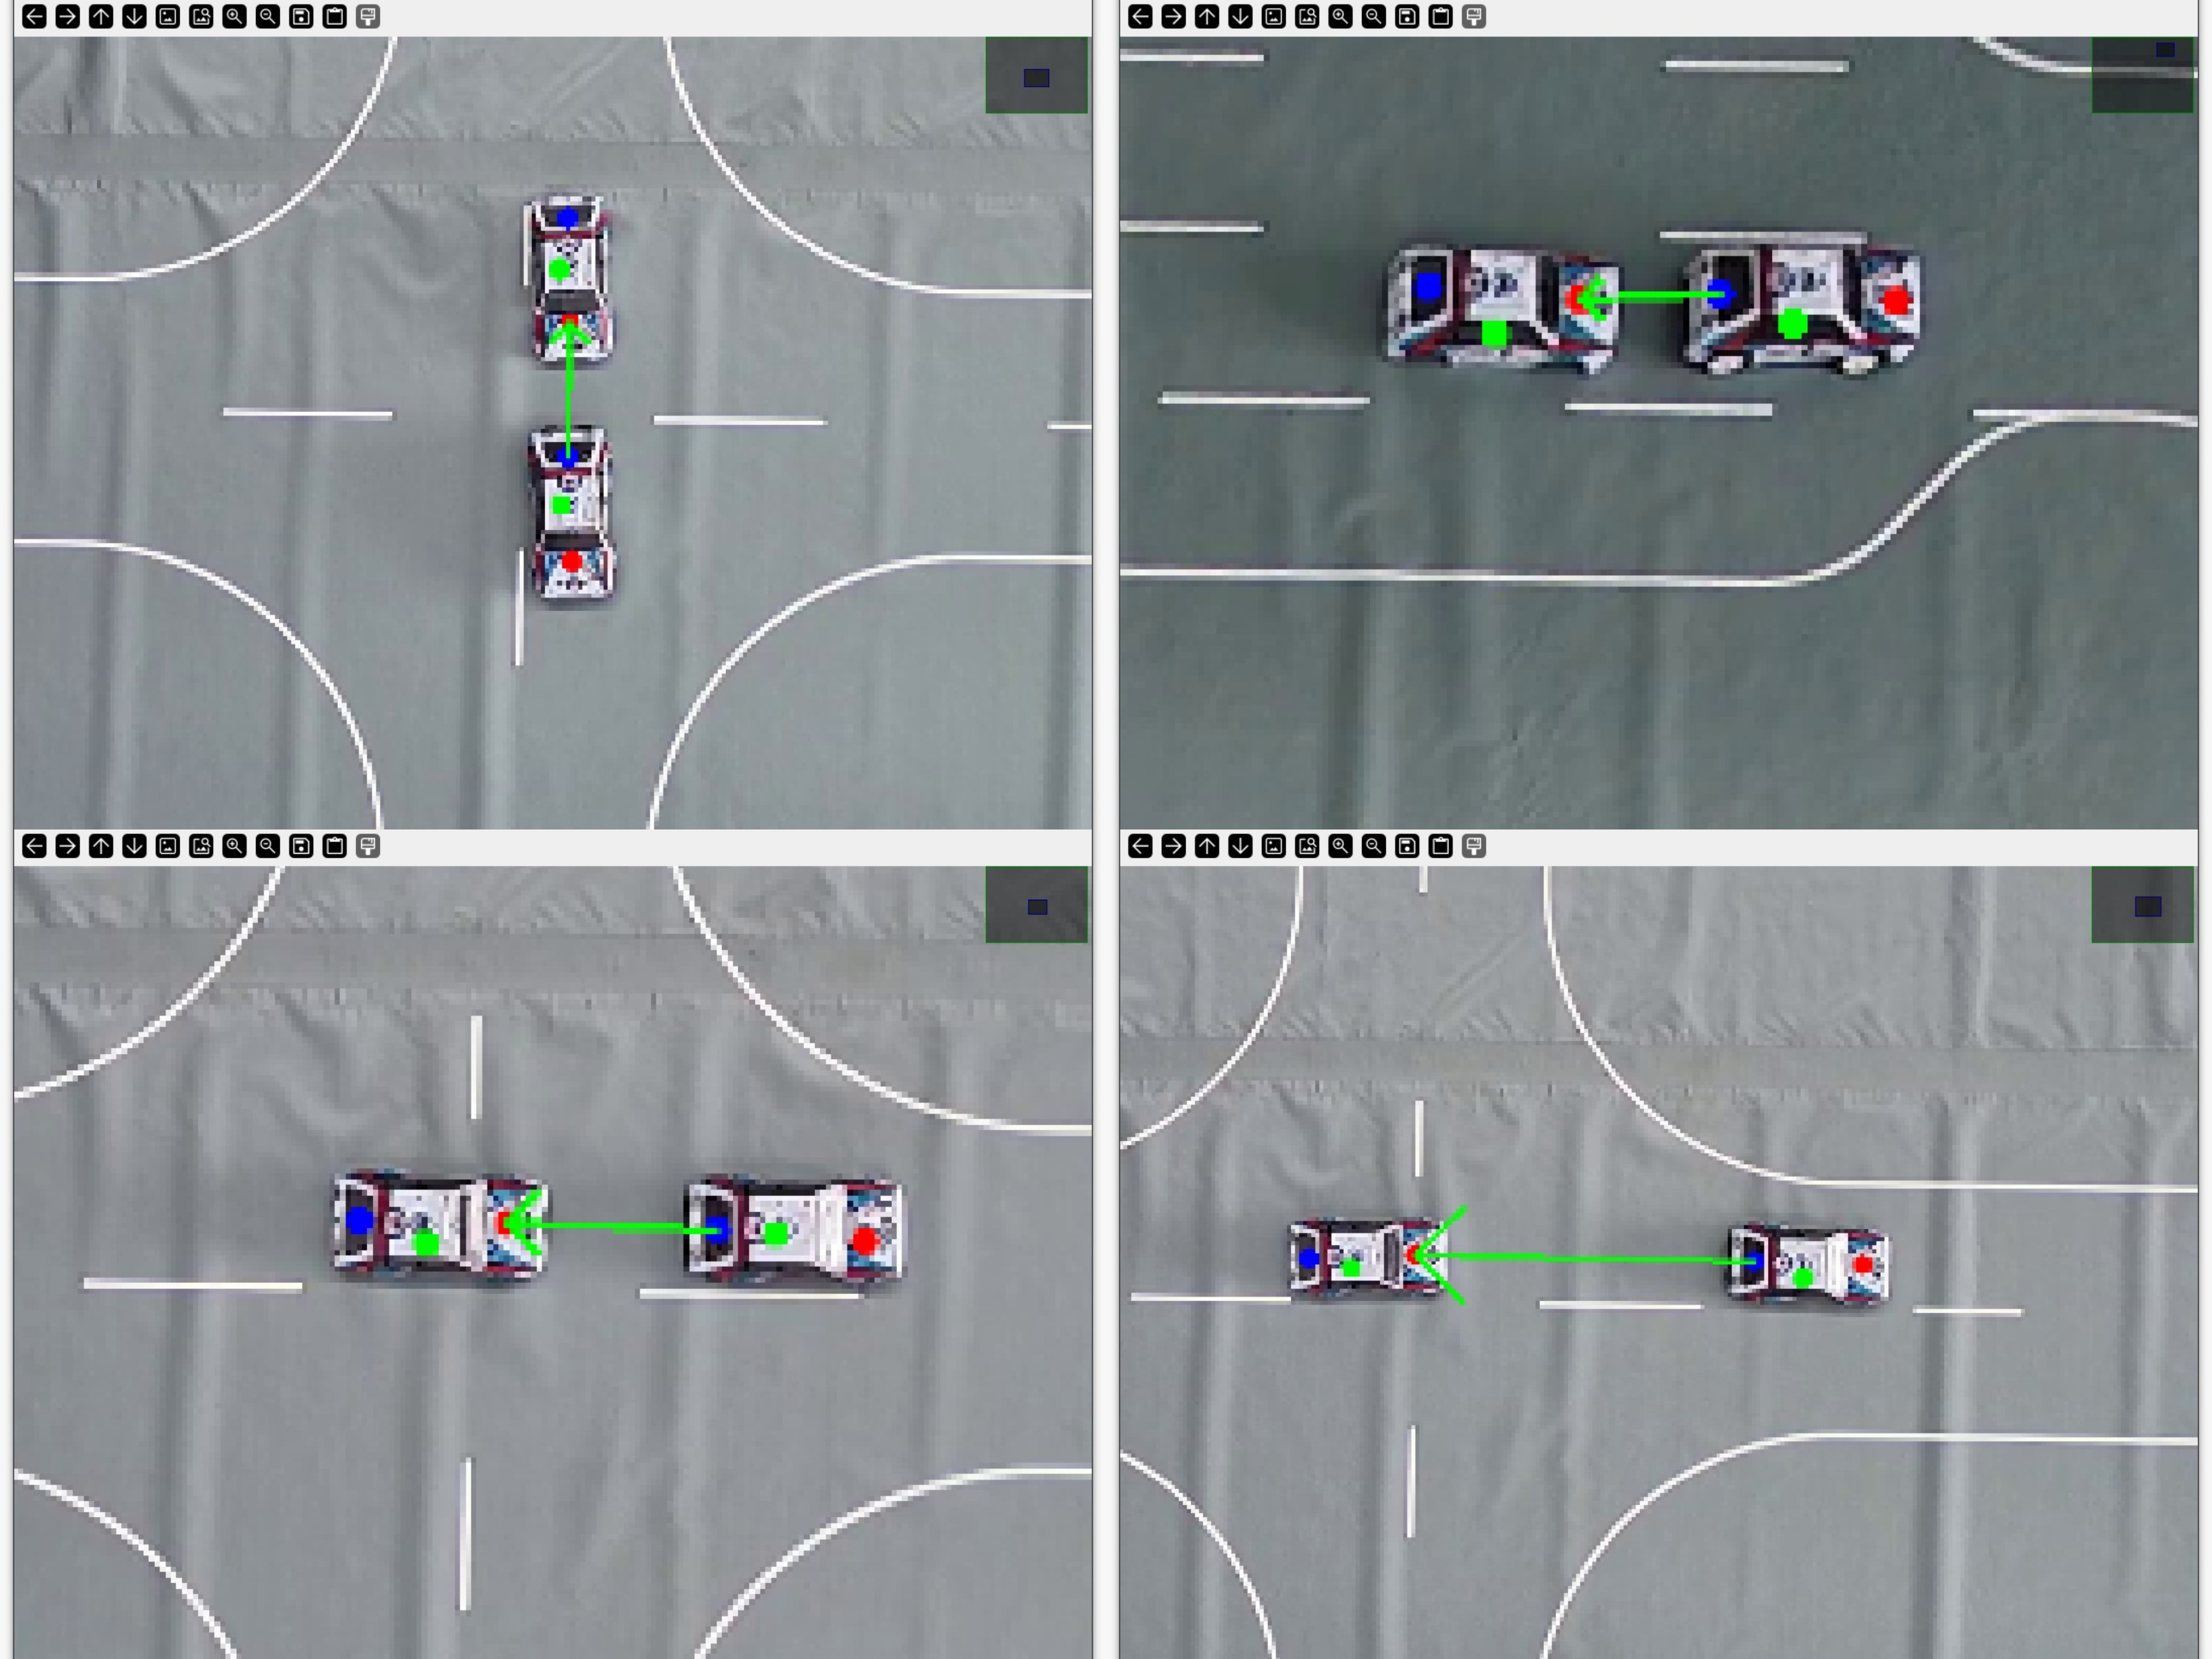
\includegraphics[width=0.95\textwidth]{figure4.61.jpg}
	\caption{Localization performance for vehicle spacing below the reliable localization threshold of 21cm, illustrating tracking ambiguity and segmentation overlap.}
	\label{fig:spacing_below}
\end{figure}

\begin{figure}[!ht]
	\centering
	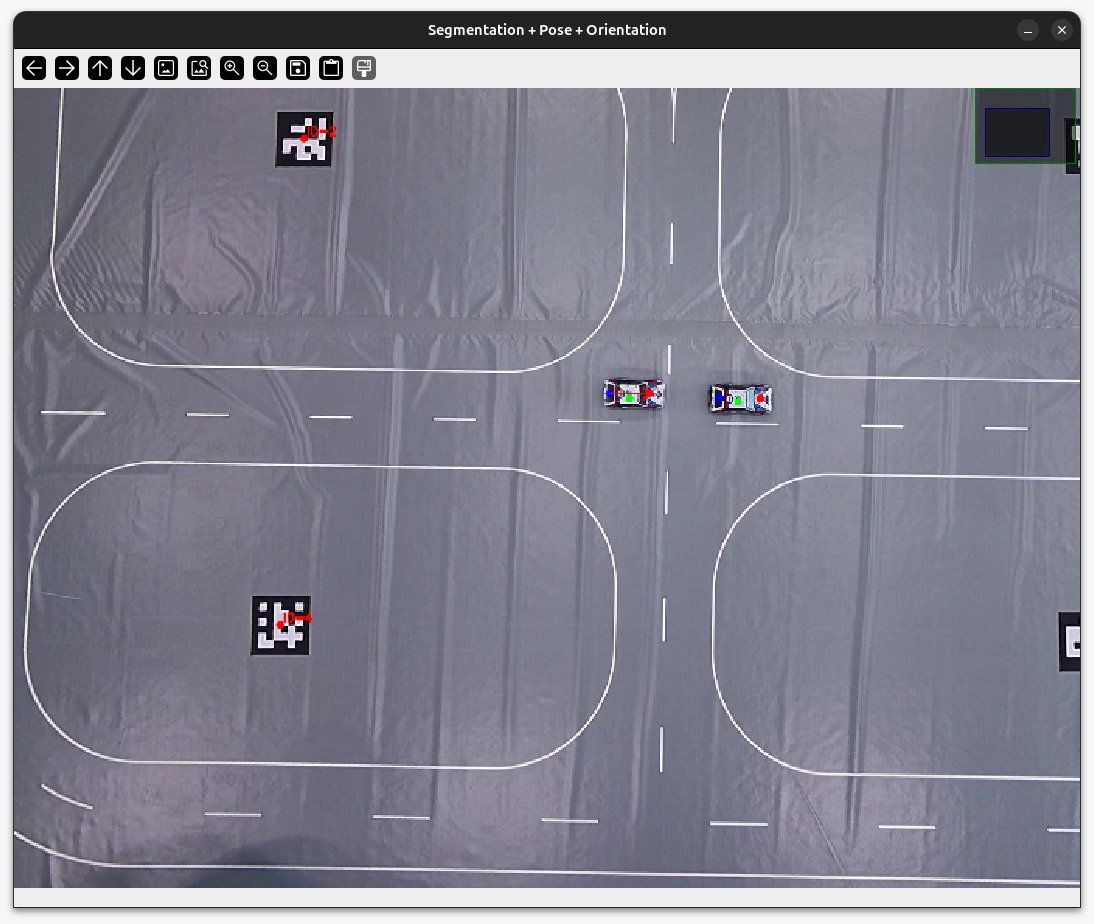
\includegraphics[width=0.95\textwidth]{figure4.62.jpeg}
	\caption{Stable localization achieved for vehicle spacing at and above the experimentally determined localization threshold of 21cm.}
	\label{fig:spacing_above}
\end{figure}
	
The computed relative positions remained stable throughout the experiments, enabling reliable estimation of inter-vehicle distance and relative heading. The framework successfully distinguished between approaching and separating vehicles while maintaining accurate localization during close-proximity interactions.

\subsection{Robustness Evaluation}

The final experiment investigates the robustness of the proposed perception framework under challenging operating conditions, including curved road navigation, close-proximity vehicle interactions, image boundary conditions, and varying illumination levels. Representative experimental results are presented in Figure~\ref{fig:robustness} and Figure~\ref{fig:lighting}.

\marginnote{
	\textbf{Robustness tests}\\
	Localization performance evaluated under varying illumination, vehicle colours, and boundary conditions.
}

\begin{figure}[!ht]
	\centering
	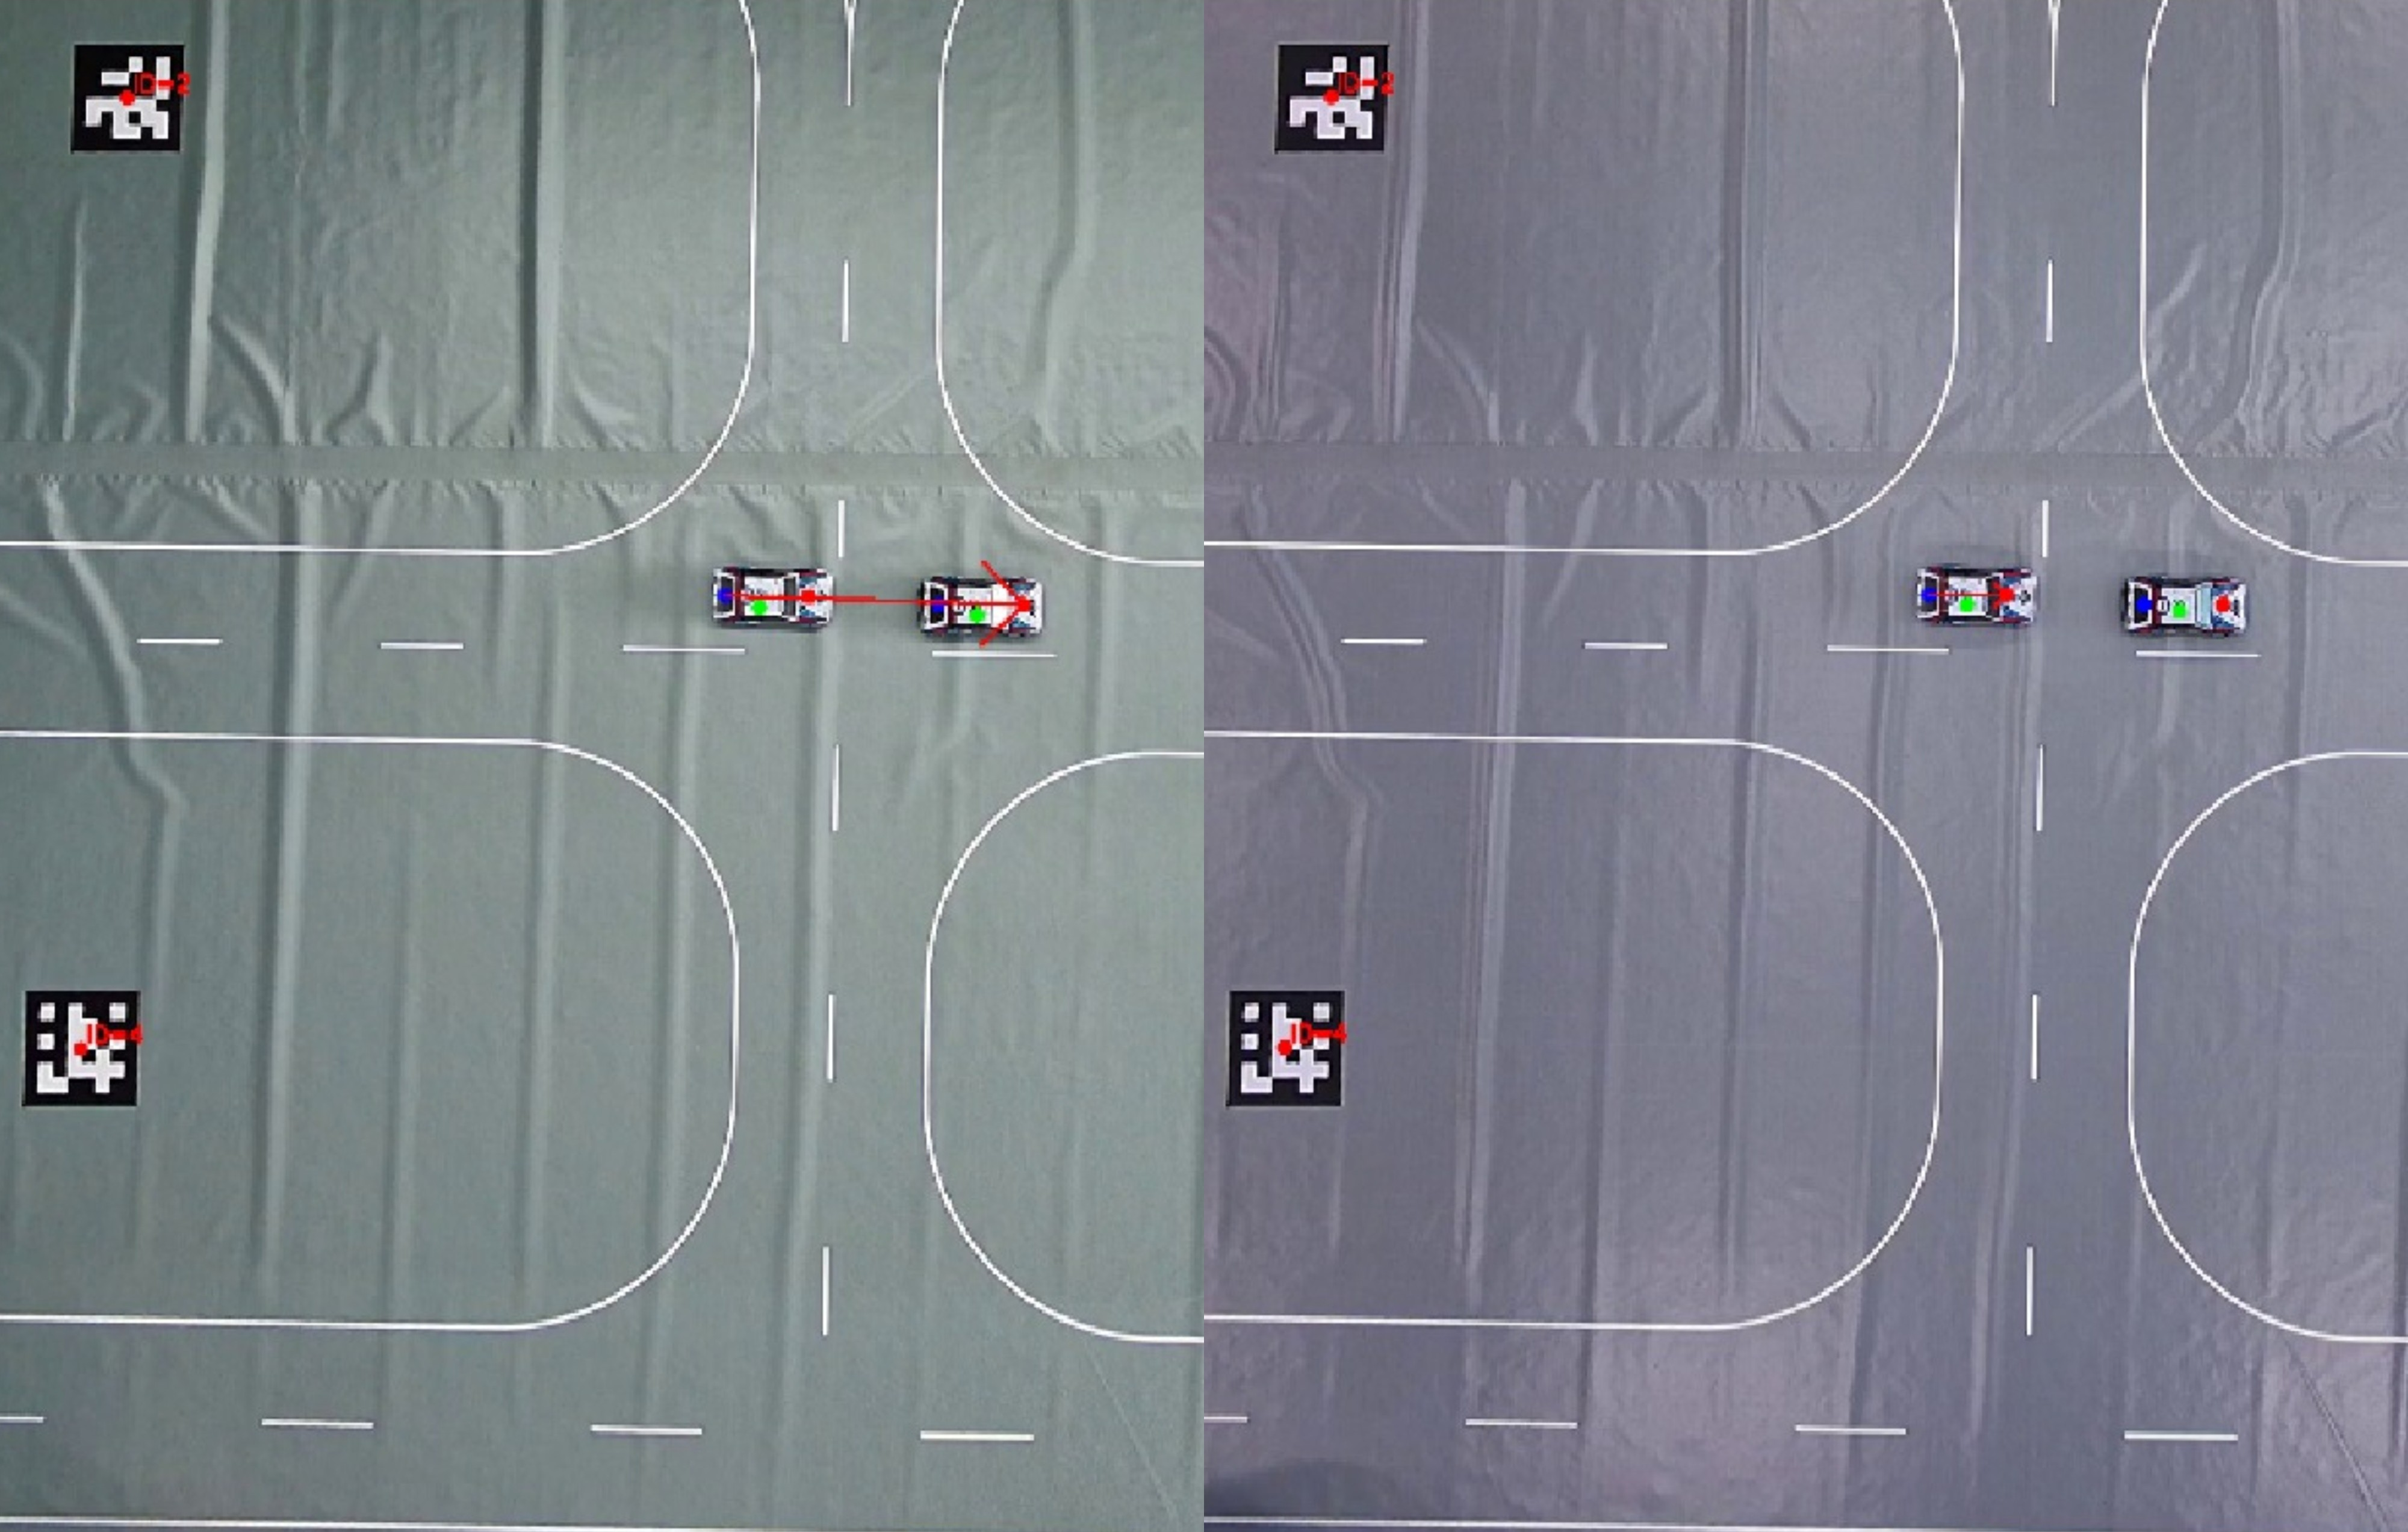
\includegraphics[width=0.95\textwidth]{figure4.71.jpg}
	\caption{Localization performance under normal and reduced illumination conditions, demonstrating robustness to lighting variations.}
	\label{fig:lighting}
\end{figure}
	
\begin{figure}[!ht]
	\centering
	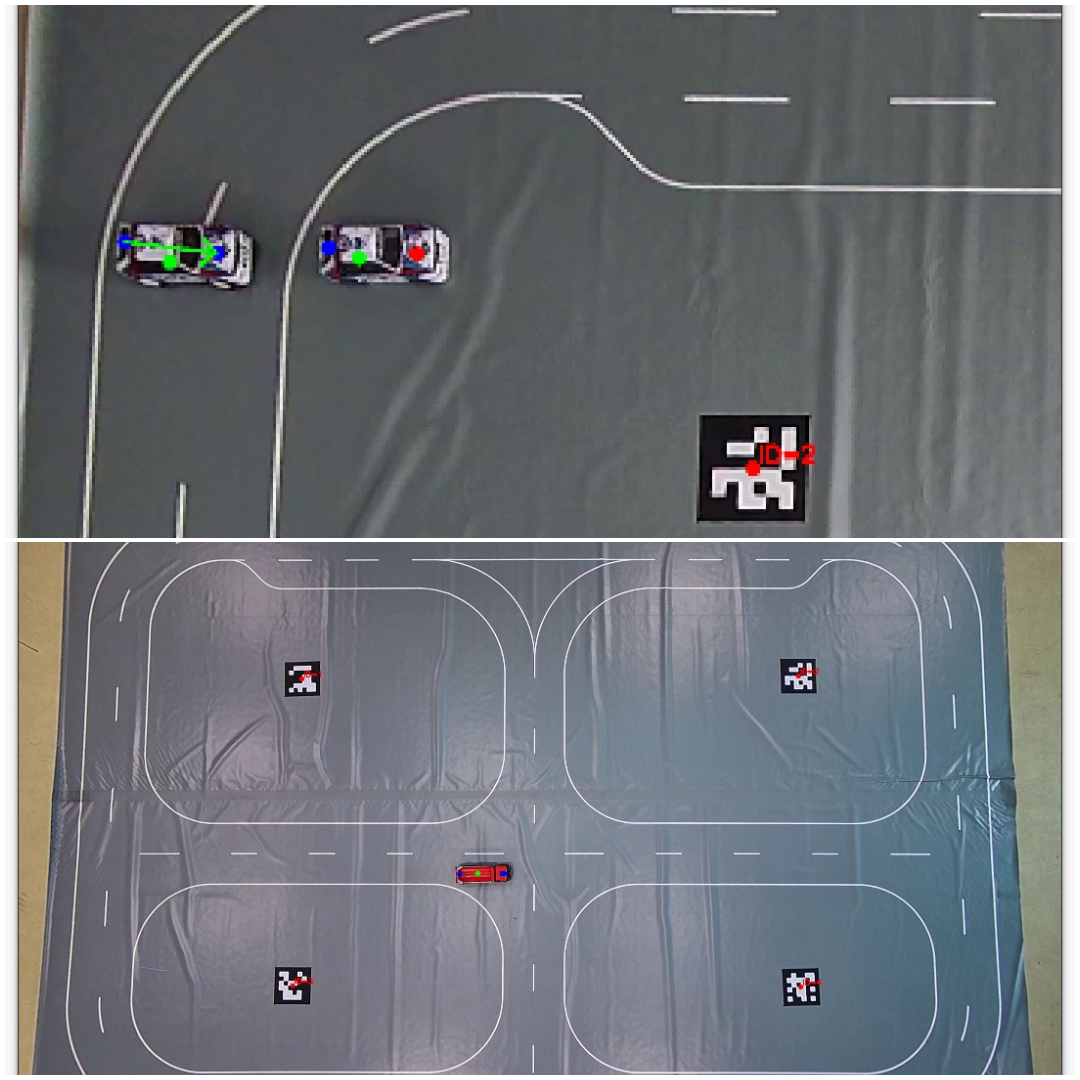
\includegraphics[width=0.90\textwidth]{figuure4.72.png}
	\caption{Localization results for different vehicle colours and representative corner-case scenarios, demonstrating robustness to appearance variations.}
	\label{fig:robustness}
\end{figure}

The proposed perception framework maintained reliable vehicle detection and pose estimation across all evaluated scenarios, including curved roads, close vehicle interactions, image boundaries, and varying lighting conditions, demonstrating robust localization performance under representative indoor operating conditions.

\section{Chapter Summary}

This chapter presented the experimental validation of the proposed Bird's-Eye View (BEV) perception framework using a miniature autonomous driving platform. The measurement campaign included both quantitative and qualitative evaluations to assess the performance of the developed vehicle detection and localization system.

The latency measurements demonstrated a consistent end-to-end processing delay of less than 250~ms across different experimental conditions, confirming that the perception pipeline satisfies the real-time requirements of the application. Furthermore, qualitative validation showed that the proposed framework accurately estimated vehicle pose, orientation, and relative position under a range of representative traffic scenarios. Reliable localization performance was maintained for single-vehicle and multi-vehicle environments, as well as under challenging conditions including curved road segments, close vehicle interactions, and image boundary regions.

Overall, the experimental results confirm that the developed perception framework provides robust and reliable localization within the miniature autonomous driving environment, establishing a solid foundation for the sensor fusion and state estimation approach presented in the following chapter.

\chapter{Implementation of Extended Kalman Filter}
\label{chap:ekf}
\section{Theory of Kalman Filters \& EKF}

The motivation of Rudolf Kalman for deriving the Kalman filters was to improve the accuracy of estimation and prediction of states using a probabilistic filter. The Kalman filter works on the principle of predicting the current states of a system based on either a static or dynamic mathematical state space model of the plant and the previously estimated state and then perform correction using current measured states. The accuracy of the filter therein lies in the appropriate physcial plant modelling and fine tuning of the relevant covariance matrices of measurement and process noise.

\subsection{State Space Systems}
The state space refers to the mathematical model of a physical system described using a set of variables which are related by first order differential or difference equation. The variables involved are known as \textbf{state variables} and the system state defined by them is called \textbf{state} in short.

\subsection{Random Noise and Probability Distributions}

Every physical phenomenon in nature can be measured using modern sensors and mechanical devices. The measurement of any state/path variable embeds a certian noise of uncertainty in the measurement campaign. This is mostly due to the accuracy of sensors. this noise is accompanied by yet another uncertainity of unmodelled disturbances, as the state of a dynamic system constantly changes with time. The mathematical approach for handling uncertainties is highlighted by probabilistic distributions. The probability curve for an ideal measurement campaign with infinite instances of data measurement tends towards a normal distribution as dictated by Central Limit Theorem. The normal distribution of any quantity is described using the mean and the standard deviation.

The linear Kalman Filter models the measurement noise and the process noise seperately and evaluated them using a factor known as Kalman Gain. this factor could show the balance or trusting tendency between measurement data point and the prediction data point. The factor is updated after every iteration of calculation and is used to update the filter matrices.

The disadvantage of Linear Kalman Filter lies in handling the state space plant models with non-linear differential equations, In EKF however the linearisation is performed dynamically around the current state estimate for every time step using first order taylor series expansion(the Jacobian matrices). This also signifies that the probability distribution of non-linear plants is also non-Gaussian and cannot be depicted using normal distribution. 

\subsection{One-Dimensional Linear Kalman Filter}
\label{sec:kalman_filter_1d}

In one-dimensional state estimation, the Kalman filter operates as a cyclic two-phase algorithm consisting of a \enquote{Predict} phase (extrapolation) and a \enquote{Correct} phase (update).~\cite{CC17}%
\sidenote{$\hat{x}_{n,n}$ denotes the current state estimate at discrete time step $n$ after taking measurement $z_n$, while $\hat{x}_{n+1,n}$ represents the predicted state for the next time step but derived at current time step. Similarly, $p_{n,n}$ is the estimate variance (uncertainty), $r_n$ is the measurement variance, and $q_n$ is the process noise variance.}

The filter is statistically optimal because it combines prior predictions and noisy sensor measurements in a manner that provably minimizes the estimation uncertainty $p_{n,n}$. The filter also requires Initial values of $\hat{x}_{0,0}$ and its variance $p_{0,0}$, Choosing an excessively high initial variance (e.g., $p_{0,0}=10{,}000$) will lead to longer convergence times, whereas setting it too low can cause estimator overconfidence

The following five equations define the complete recursive loop for a linear system:

\begin{enumerate}[label=\textbf{Step \arabic*:}, leftmargin=*, itemsep=1em]
	
	\item \textbf{State Extrapolation (\emph{Predict})}\\
	This step extrapolates the current system state estimate forward to the next time step/iteration cycle using the governing dynamic model of the plant. For constant velocity dynamics, the position advances by the estimated velocity multiplied by the time interval $\Delta t$, while velocity remains constant.
	\begin{equation}
		\begin{split}
			&\hat{x}_{n+1,n} = \hat{x}_{n,n} + \Delta t \hat{\dot{x}}_{n,n} \\ 
			& (\text{or } \hat{x}_{n+1,n} = \hat{x}_{n,n} \text{ for constant dynamics})
		\end{split}
	\end{equation}
	
	\item \textbf{Covariance Extrapolation (\emph{Predict})}\\
	This step extrapolates the estimate variance ahead in time to account for uncertainty introduced during the transition interval.%
	\sidenote{Alternative literature designations for process noise variance $q_n$ include plant noise, driving noise, dynamics noise, model noise, and system noise.}\\
	Combines the baseline uncertainty of the current estimate with the additive process noise variance ($q_n$).
	\begin{equation}
		\begin{split}
			&p_{n+1,n} = p_{n,n} + q_n \\ 
			& (\text{or } p_{n+1,n}^x = p_{n,n}^x + \Delta t^2 p_{n,n}^v + q_n \text{ for constant velocity})
		\end{split}
	\end{equation}
	
	\item \textbf{Kalman Gain (\emph{Update})}\\
	Then compute the optimal weighting coefficient between zero and one that balances trust between the prior prediction and the new sensor data.\\
	 It evaluates the ratio of the prior extrapolated estimate variance against the total system uncertainty, including measurement variance ($r_n$).
	\begin{equation}
		K_n = \frac{p_{n,n-1}}{p_{n,n-1} + r_n}
	\end{equation}
	
	\item \textbf{State Update (\emph{Update})}\\
	Now refine the prior state estimate by incorporating the actual sensor measurement ($z_n$) sampled at the current cycle.\\
	Adjusts the prior prediction by the measurement residual (innovation), scaled precisely by the calculated Kalman Gain.
	\begin{equation}
		\hat{x}_{n,n} = \hat{x}_{n,n-1} + K_n\left(z_n - \hat{x}_{n,n-1}\right)
	\end{equation}
	
	\item \textbf{Covariance Update (\emph{Update})}\\
	Finally update the estimate variance of the current state to reflect the reduction in uncertainty after consuming the measurement.%
	\sidenote{Because $(1 - K_n) \le 1$, the estimate variance $p_{n,n}$ strictly decreases during each update, driving the filter toward steady-state convergence.}\\
	Scales the prior extrapolated variance down by the complementary factor $(1 - K_n)$ to ensure estimator convergence over time.
	\begin{equation}
		p_{n,n} = (1 - K_n)p_{n,n-1}
	\end{equation}
	
\end{enumerate}


\paragraph{Extension to Non-Linear Systems: The Extended Kalman Filter}
\label{sec:extended_kalman_filter}

When the underlying system dynamics or sensor relationships are non-linear, the simple scalar arithmetic is generalized into the Extended Kalman Filter (\textsc{Ekf}).%
\sidenote{To propagate estimate uncertainties through non-linearities without distortion, the \textsc{EKF} applies a first-order Taylor series expansion around the current estimate, generating partial derivative slope terms (Jacobians).}
the linear steps are replaced by introducing non-linear state and measurement functions, $f(\cdot)$ and $h(\cdot)$, alongside their respective \textbf{Jacobian derivatives, $F_n$ and $H_n$.}


\begin{enumerate}[label=\textbf{Step \arabic*:}, leftmargin=*, itemsep=1em]
	
	\item \textbf{Non-Linear State Extrapolation (\emph{Predict})}\\
	Extrapolates the state estimate directly through the non-linear dynamic model function $f(\cdot)$ using known control inputs $u_n$.
	\begin{equation}
		\hat{x}_{n+1,n} = f\left(\hat{x}_{n,n}, u_n\right)
	\end{equation}
	
	\item \textbf{Linearized Covariance Extrapolation (\emph{Predict})}\\
	Propagates the estimate variance using the dynamic model Jacobian slope $F_n$, evaluated at the current state estimate, plus process noise variance $q_n$.
	\begin{equation}
		p_{n+1,n} = F_n p_{n,n} F_n^\top + q_n \; \text{where} \; F_n = \left. \frac{\partial f}{\partial x} \right|_{\hat{x}_{n,n}, u_n}
	\end{equation}
	
	\item \textbf{Kalman Gain (\emph{Update})}\\
	Computes the optimal weighting coefficient by substituting the linearized measurement Jacobian slope $H_n$ into the variance ratio.
	\begin{equation}
		K_n = p_{n,n-1} H_n^\top \left(H_n p_{n,n-1} H_n^\top + r_n\right)^{-1} \quad \text{where} \quad H_n = \left. \frac{\partial h}{\partial x} \right|_{\hat{x}_{n,n-1}}
	\end{equation}
	
	\item \textbf{Non-Linear State Update (\emph{Update})}\\
	Refines the prior prediction by evaluating the measurement residual (innovation) directly against the non-linear measurement function $h(\cdot)$.
	\begin{equation}
		\hat{x}_{n,n} = \hat{x}_{n,n-1} + K_n\left(z_n - h\left(\hat{x}_{n,n-1}\right)\right)
	\end{equation}
	
	\item \textbf{Linearized Covariance Update (\emph{Update})}\\
	Updates the current estimate variance using the measurement Jacobian slope $H_n$ scaled by the Kalman Gain.
	\begin{equation}
		p_{n,n} = \left(I - K_n H_n\right) p_{n,n-1}
	\end{equation}
	
\end{enumerate}

\section{Non-linear Bicycle Model}
\label{sec:bicycle_model}

To accurately track and predict the vehicle's state within the Extended Kalman Filter (\textsc{EKF}), we implement a non-linear kinematic bicycle model.%
\sidenote{In a kinematic bicycle model, the two front wheels and two rear wheels are lumped together into a single steerable front wheel and a fixed rear wheel, reducing the vehicle geometry to a bicycle representation.}
\begin{marginfigure}[4\baselineskip] % Positive number pushes it down below the text!
	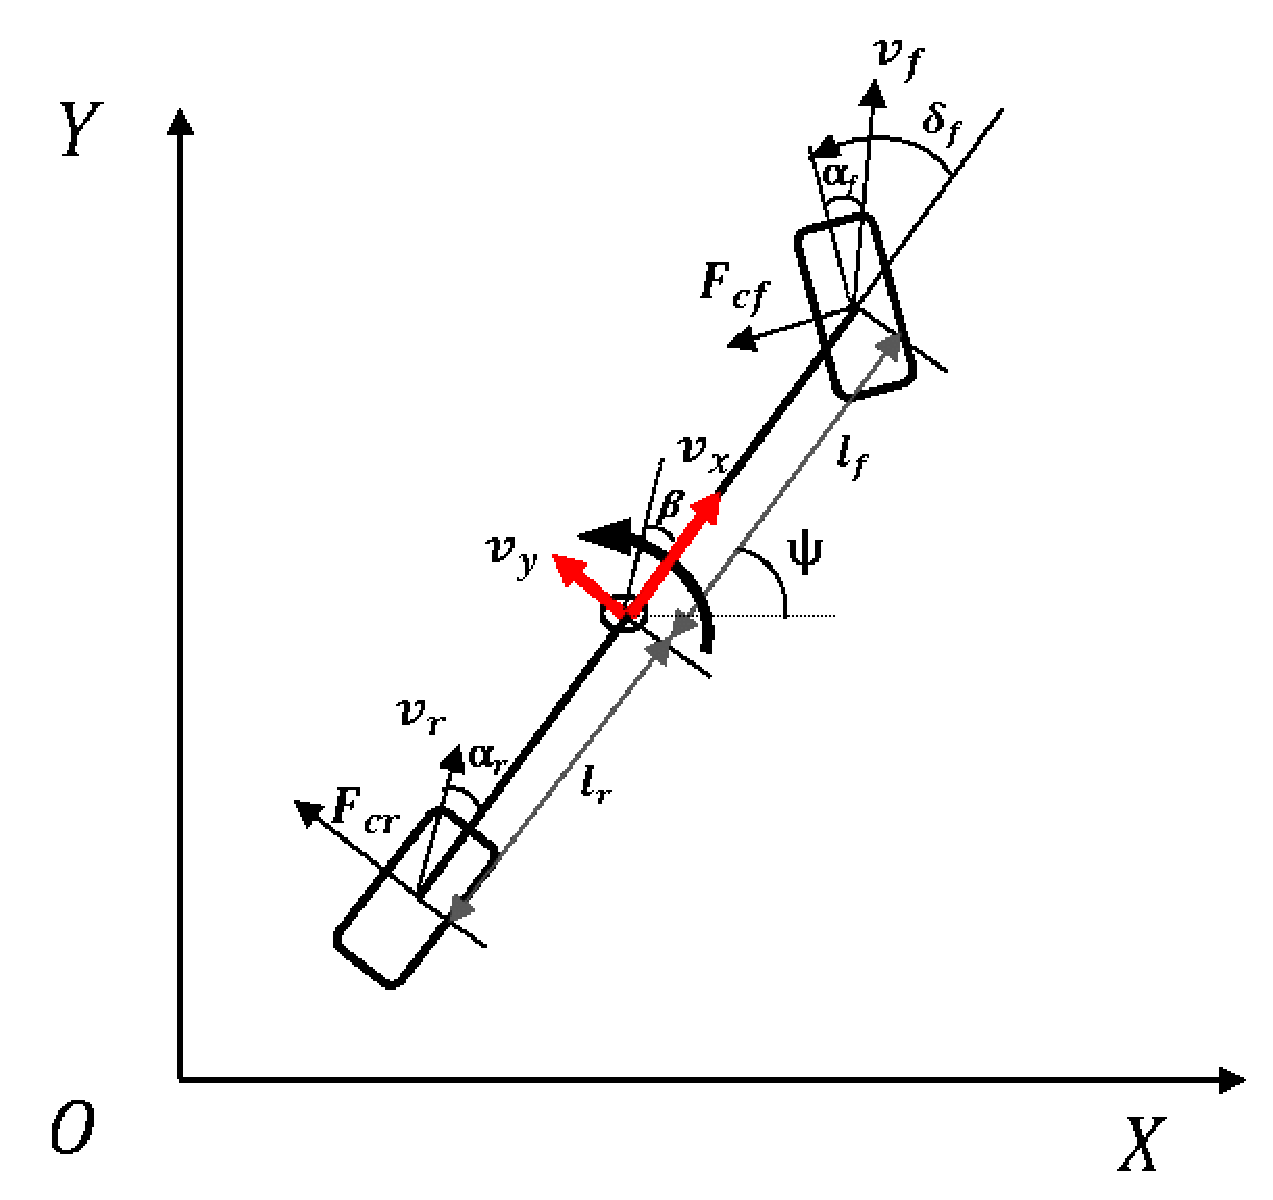
\includegraphics[width=0.9\marginparwidth]{dynamic-bicycle-model.pdf}~\cite{bicyclemodel}
	\caption{\label{fig:dynamic_bicycle}Dynamic bicycle model.}
\end{marginfigure}
Specifically, we utilize a Constant Turn Rate Velocity (\textsc{Ctrv}) (\Cref{sec:ctrv_theory}) assumption, which defines the state vector across five variables: X-position, Y-position, yaw angle, longitudinal velocity, and yaw rate.

We prioritize the CTRV model over simpler linear approximations (such as the Constant Velocity model) due to to following reasons -

\begin{enumerate}[label=\textbf{Reason \arabic*:}, leftmargin=*, itemsep=1em]
	\item \textbf{Superiority over Linear models :} When a vehicle executes a turn (e.g., a roundabout or highway lane change), a CV model interprets the lateral curve as massive unmodeled process noise. This causes lag, high estimation errors, and potential track loss. CTRV anticipates the curvature, keeping the Kalman Gain stable.
	
	\item \textbf{Vehicle Agnostic \& Kinematic Stability :} A dynamic model requires knowledge of the vehicle parameters like slip angle, cornering stiffness and road friction coefficients, CTRV is strictly kinematic and its state variables are observable which is highly relevant for a vision based tracking system without any vehicle knowledge
	
	\item \textbf{Architectural Flexibility :}This architectural flexibility allows the state transition model to generalize seamlessly across both high-speed straightaways and highly dynamic urban navigation without requiring real-time parameter tuning or model switching
\end{enumerate}
	

The implementation of the prediction and update loops using this non-linear formulation is presented in Listing~\ref{lst:ekf_tracker}.

\begin{lstlisting}[language=Python, float=t, escapechar=, basicstyle=\footnotesize\ttfamily, aboveskip=0.5em, belowskip=0.5em, caption={Implementation of the Extended Kalman Filter using a non-linear CTRV bicycle model for state tracking.}, label={lst:ekf_tracker}]
	import numpy as np
	
	class EKFTracker:
	def __init__(self, dt):
	self.dt = dt
	self.x = np.zeros((5, 1))
	self.P = np.eye(5) 
	self.Q = np.diag([0.1, 0.1, np.deg2rad(1.0), 1.0, np.deg2rad(1.0)])**2
	self.R = np.diag([2.0, 2.0, np.deg2rad(5.0)])**2 
	self.H = np.array([[1, 0, 0, 0, 0], [0, 1, 0, 0, 0], [0, 0, 1, 0, 0]])
	
	def predict(self):
	x, y, theta, v, omega = self.x.flatten()
	dt, sin_t, cos_t = self.dt, np.sin(theta), np.cos(theta)
	
	if abs(omega) > 0.001:
	sin_to, cos_to = np.sin(theta + omega * dt), np.cos(theta + omega * dt)
	v_w, v_w2 = v / omega, v / (omega ** 2)
	self.x[0, 0] = x + v_w * (sin_to - sin_t)
	self.x[1, 0] = y + v_w * (-cos_to + cos_t)
	self.x[2, 0] = theta + omega * dt
	self.x[3, 0], self.x[4, 0] = v, omega  
	
	f02, f12 = v_w * (cos_to - cos_t), v_w * (sin_to - sin_t)
	f03, f13 = (sin_to - sin_t) / omega, (-cos_to + cos_t) / omega
	f04 = (dt * v_w * cos_to) - v_w2 * (sin_to - sin_t)
	f14 = (dt * v_w * sin_to) - v_w2 * (-cos_to + cos_t)
	else:
	self.x[0, 0], self.x[1, 0] = x + v * cos_t * dt, y + v * sin_t * dt
	self.x[2, 0] = theta + omega * dt
	self.x[3, 0], self.x[4, 0] = v, omega  
	
	f02, f12 = -v * sin_t * dt, v * cos_t * dt
	f03, f13 = cos_t * dt, sin_t * dt
	f04, f14 = -0.5 * v * (dt**2) * sin_t, 0.5 * v * (dt**2) * cos_t
	
	F = np.array([[1, 0, f02, f03, f04], [0, 1, f12, f13, f14],
	[0, 0, 1, 0, dt], [0, 0, 0, 1, 0], [0, 0, 0, 0, 1]])
	self.P = F @ self.P @ F.T + self.Q
	
	def update(self, z):
	y_res = z - (self.H @ self.x)
	y_res[2, 0] = (y_res[2, 0] + np.pi) % (2 * np.pi) - np.pi
	S = self.H @ self.P @ self.H.T + self.R
	K = self.P @ self.H.T @ np.linalg.inv(S)
	self.x = self.x + (K @ y_res)
	self.P = (np.eye(5) - K @ self.H) @ self.P
\end{lstlisting}



\subsection{Constant Turn Rate and Velocity (CTRV) Model}
\label{sec:ctrv_theory}

The Constant Turn Rate and Velocity (\textsc{Ctrv}) model is a non-linear kinematic motion model widely utilized for vehicular state estimation and object tracking.%
\sidenote{Unlike simpler models that assume rectilinear motion, the \textsc{Ctrv} model explicitly accounts for curved trajectories by assuming that both the resultant velocity magnitude and the turn rate remain constant over a discrete time step $\Delta t$.}
The mathematical formulation of the model is structured into its state representation, continuous dynamics, and discrete-time integration.

\paragraph{State Space Representation}
The system state is defined by a five-dimensional vector representing the vehicle's kinematics in a two-dimensional Cartesian plane:
\begin{equation}
	\mathbf{x} = [x, \, y, \, \theta, \, v, \, \omega]^\top
	\label{eq:ctrv_state}
\end{equation}
where the individual state variables represent the following physical quantities:
\begin{itemize}
	\item $x, y$: Spatial coordinates of the vehicle's reference point (typically the center of gravity or rear axle).
	\item $\theta$: Yaw angle (orientation or heading) relative to the X-axis.
	\item $v$: Resultant longitudinal velocity magnitude ($\sqrt{\dot{x}^2 + \dot{y}^2}$).
	\item $\omega$: Yaw rate ($\dot{\theta}$, representing the angular velocity of the heading).
\end{itemize}

\paragraph{Continuous-Time Differential Dynamics}
The core assumption of the \textsc{Ctrv} model is that the longitudinal acceleration ($\dot{v}$) and angular acceleration ($\dot{\omega}$) are strictly zero over the transition interval. Consequently, the continuous-time differential equations governing the kinematic system are expressed as:
\begin{align}
	\dot{x}(t) &= v(t) \cos(\theta(t)) \\
	\dot{y}(t) &= v(t) \sin(\theta(t)) \\
	\dot{\theta}(t) &= \omega(t) \\
	\dot{v}(t) &= 0 \\
	\dot{\omega}(t) &= 0
\end{align}

\paragraph{Discrete-Time State Transition}
To implement these continuous dynamics within a recursive discrete-time filter such as the Extended Kalman Filter (\textsc{Ekf}), the differential equations must be integrated from time step $n$ to $n+1$ over the interval $\Delta t$. Because the heading angle changes continuously as $\theta(t) = \theta_n + \omega_n \tau$ during a turn, integrating the position rates requires evaluating:
\begin{align}
	x_{n+1} &= x_n + \int_0^{\Delta t} v_n \cos(\theta_n + \omega_n \tau) \, d\tau \\
	y_{n+1} &= y_n + \int_0^{\Delta t} v_n \sin(\theta_n + \omega_n \tau) \, d\tau
\end{align}
Evaluating these analytical integrals yields two distinct operational regimes based on the rotational velocity:


\begin{enumerate}[label=\textbf{Case \Alph*:}, leftmargin=*, itemsep=1em]
	
	\item \textbf{Non-Zero Turn Rate ($\omega_n \neq 0$)}\\
	When the vehicle is actively turning, exact analytical integration of the continuous-time equations yields:
	\begin{align}
		x_{n+1} &= x_n + \frac{v_n}{\omega_n} \left( \sin(\theta_n + \omega_n \Delta t) - \sin(\theta_n) \right) \\
		y_{n+1} &= y_n + \frac{v_n}{\omega_n} \left( -\cos(\theta_n + \omega_n \Delta t) + \cos(\theta_n) \right) \\
		\theta_{n+1} &= \theta_n + \omega_n \Delta t \\
		v_{n+1} &= v_n \\
		\omega_{n+1} &= \omega_n
	\end{align}
	
	\item \textbf{The Singularity Case ($\omega_n = 0$)}\\
	If the vehicle travels in a straight line, $\omega_n \to 0$, introducing a division-by-zero singularity ($\frac{v_n}{0}$) in the non-linear position equations. Applying L'H\^{o}pital's rule (or integrating directly with a constant $\theta_n$) collapses the transition model cleanly into the standard Constant Velocity (\textsc{Cv}) equations:
	\begin{align}
		x_{n+1} &= x_n + v_n \cos(\theta_n) \Delta t \\
		y_{n+1} &= y_n + v_n \sin(\theta_n) \Delta t \\
		\theta_{n+1} &= \theta_n \\
		v_{n+1} &= v_n \\
		\omega_{n+1} &= 0
	\end{align}
	
\end{enumerate}

\section{Tuning of Q and R Matrices}
\label{sec:tuning_q_r}

The performance and numerical stability of the Extended Kalman Filter (\textsc{Ekf}) depends fundamentally on the ratio between the process noise covariance matrix $\mathbf{Q}$ and the measurement noise covariance matrix $\mathbf{R}$.%
\sidenote{The ratio between $\mathbf{Q}$ and $\mathbf{R}$ directly dictates the weighting of the Kalman Gain. If $\mathbf{Q} \ll \mathbf{R}$, the filter places high trust in the mathematical dynamic model, resulting in smooth trajectories but sluggish reaction times during sudden maneuvers. Conversely, if $\mathbf{Q} \gg \mathbf{R}$, the filter trusts incoming sensor data over the model, reacting rapidly to trajectory changes at the expense of passing sensor jitter directly into the state estimates.}
While the theoretical equations of the filter assume these covariance matrices are precisely known, obtaining their true real-world values requires a structured empirical methodology rather than arbitrary guessing.

\subsection{Best Practices for Filter Tuning}

Establishing an optimal filter architecture requires treating measurement noise and process noise through two distinct analytical paradigms: static quantification and dynamic evaluation.

\paragraph{Empirical Determination of Measurement Noise ($\mathbf{R}$)}
Because $\mathbf{R}$ represents the physical inaccuracies and environmental uncertainty of the sensor pipeline (such as camera quantization, detection jitter, or spatial calibration errors in a YOLO object detection framework), best practice dictates that it should never be estimated by trial and error. Instead, $\mathbf{R}$ should be established empirically through a static measurement campaign.%

By placing the target vehicle at known, stationary test coordinates and logging raw sensor observations to CSV files over extended periods, one can statistically quantify the sensor's behavior. Calculating the sample variance $\sigma^2$ across the stationary time-series data provides a mathematically rigorous, ground-truth anchor for the diagonal elements of $\mathbf{R}$.

\paragraph{Dynamic Evaluation of Process Noise ($\mathbf{Q}$)}
Unlike sensor noise, the process noise covariance $\mathbf{Q}$ represents unmodeled system dynamics—such as sudden driver steering inputs, road banking, or transient acceleration spikes that deviate from the Constant Turn Rate and Velocity (\textsc{Ctrv}) assumptions. Because these dynamic discrepancies only occur when the vehicle is actively moving, $\mathbf{Q}$ cannot be determined statically. 

The theoretical best practice for evaluating $\mathbf{Q}$ relies on analyzing the innovation residuals $\mathbf{y}_n$, defined as the discrepancy between the incoming sensor measurement $\mathbf{z}_n$ and the \emph{a priori} model prediction:%
\sidenote{In a perfectly tuned filter, the innovation residuals should behave as continuous zero-mean white noise. If the residual curve exhibits systematic bias, persistent offsets, or sharp lag spikes during maneuvers, the model is under-responding, indicating that the corresponding diagonal terms in $\mathbf{Q}$ must be increased.}
\begin{equation}
	\mathbf{y}_n = \mathbf{z}_n - \mathbf{H} \hat{\mathbf{x}}_{n,n-1}
	\label{eq:innovation_residual}
\end{equation}

\subsection{Interactive GUI-Based Tuning Methodology}

In our implementation, we bridged the gap between theoretical residual analysis and practical filter optimization by developing an interactive, data-driven tuning framework. While Root Mean Square Error (\textsc{Rmse}) metrics over static test points provided our initial baseline, optimizing the filter for high-speed dynamic maneuvers required real-time visibility into the error dynamics.

To achieve this, we first locked the measurement covariance $\mathbf{R}$ using the empirical variances calculated from our static CSV measurement campaigns. Next, rather than relying on tedious offline trial-and-error to find $\mathbf{Q}$, we constructed a graphical user interface (\textsc{Gui}) using OpenCV trackbars as interactive virtual \enquote{knobs} mapped directly to the diagonal elements of the process noise matrix.

This interface was coupled with a real-time visualization tool that continuously plotted the innovation residual curve $\mathbf{y}_n$ as a live line graph during vehicle operation.%
\marginnote{\textbf{Practical Advantage:} Live visual feedback of the residual line graph allows the engineer to instantly distinguish between sensor noise spikes and true kinematic lag, making it possible to find the exact convergence sweet-spot in minutes rather than hours.}
While the vehicle executed dynamic test maneuvers—such as sharp turns and rapid linear accelerations—we manually manipulated the GUI trackbars. By visually monitoring the live residual line graph, we dynamically tuned the knobs until the error curve converged to a tightly bounded, zero-mean baseline: effectively flattening systematic lag spikes during sharp turns without introducing high-frequency measurement jitter during straightaway navigation.

\section{Empirical Evaluation of EKF Smoothening}
\label{sec:ekf_evaluation}

To quantify the operational efficacy of the tuned Extended Kalman Filter (\textsc{Ekf}), telemetry data comprising $387$ frame transitions was logged during dynamic vehicular navigation. A critical performance criterion for non-linear state estimation is the filter's behavior across varying velocity regimes.%
\sidenote{In vision-based object tracking, high vehicular velocities exacerbate sensor inaccuracies due to motion blur, detection latency, and frame-to-frame bounding box quantization errors. An optimally tuned filter must dynamically increase its spatial corrections to reject these unphysical anomalies.}


% --- Figure 1: Linear Regression ---
\begin{figure}[t]
	\centering
	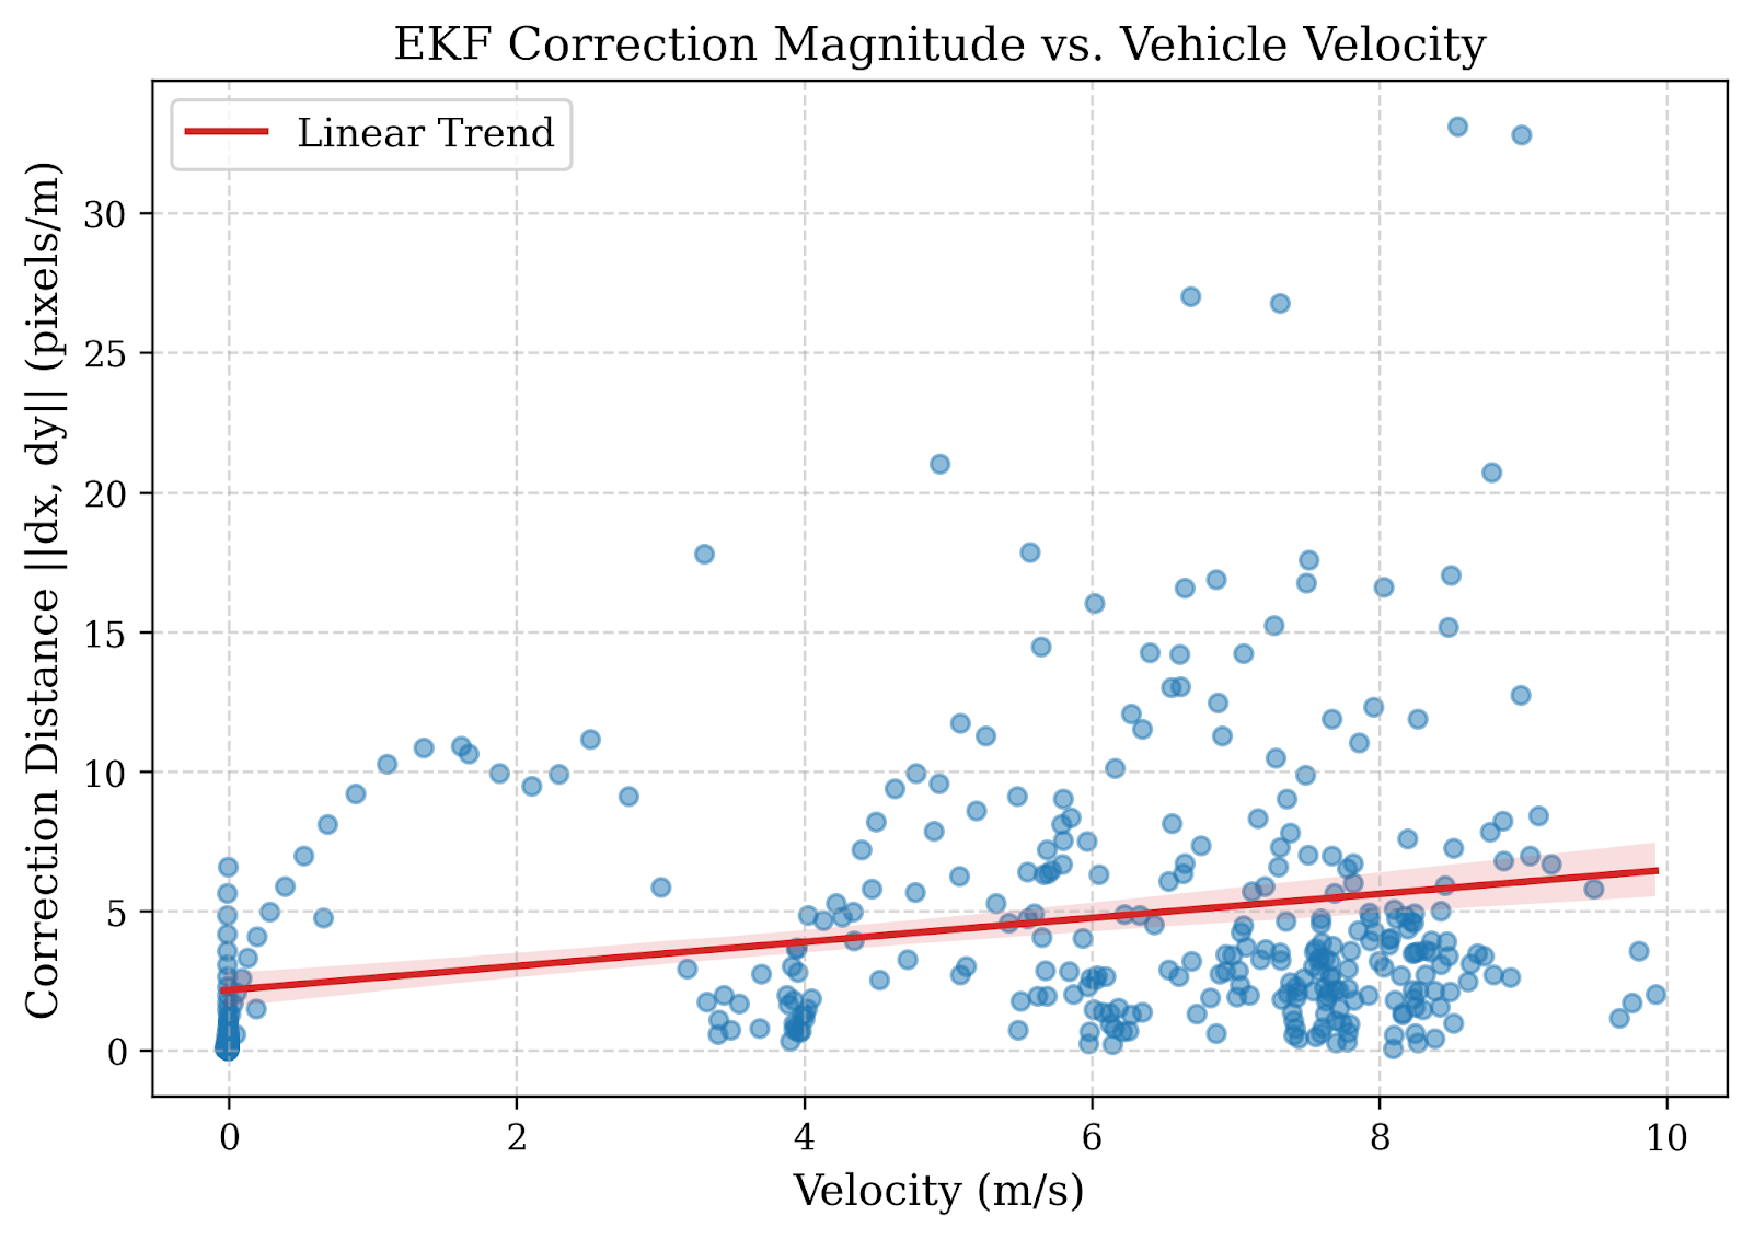
\includegraphics[width=0.8\textwidth]{figures/ekf_fig1_regression.pdf}
	\caption{\label{fig:ekf_regression}Linear regression analysis confirming a statistically significant positive correlation between vehicle velocity and EKF spatial correction magnitude $\Delta r = \|\mathbf{x}_{\text{smooth}} - \mathbf{x}_{\text{raw}}\|$.}
\end{figure}

As demonstrated in Figure~\ref{fig:ekf_regression}, the Euclidean correction distance $\Delta r = \sqrt{dx^2 + dy^2}$ exhibits a strong positive dependence on vehicle velocity. At low navigation speeds ($<2.5\text{ m/s}$), the median correction is only $0.43\text{ pixels/m}$, reflecting minor static background noise. However, as speed increases, the filter actively steps in to suppress dynamic vision errors.

% --- Figure 2: Boxplot Across Regimes ---
\begin{figure}[t]
	\centering
	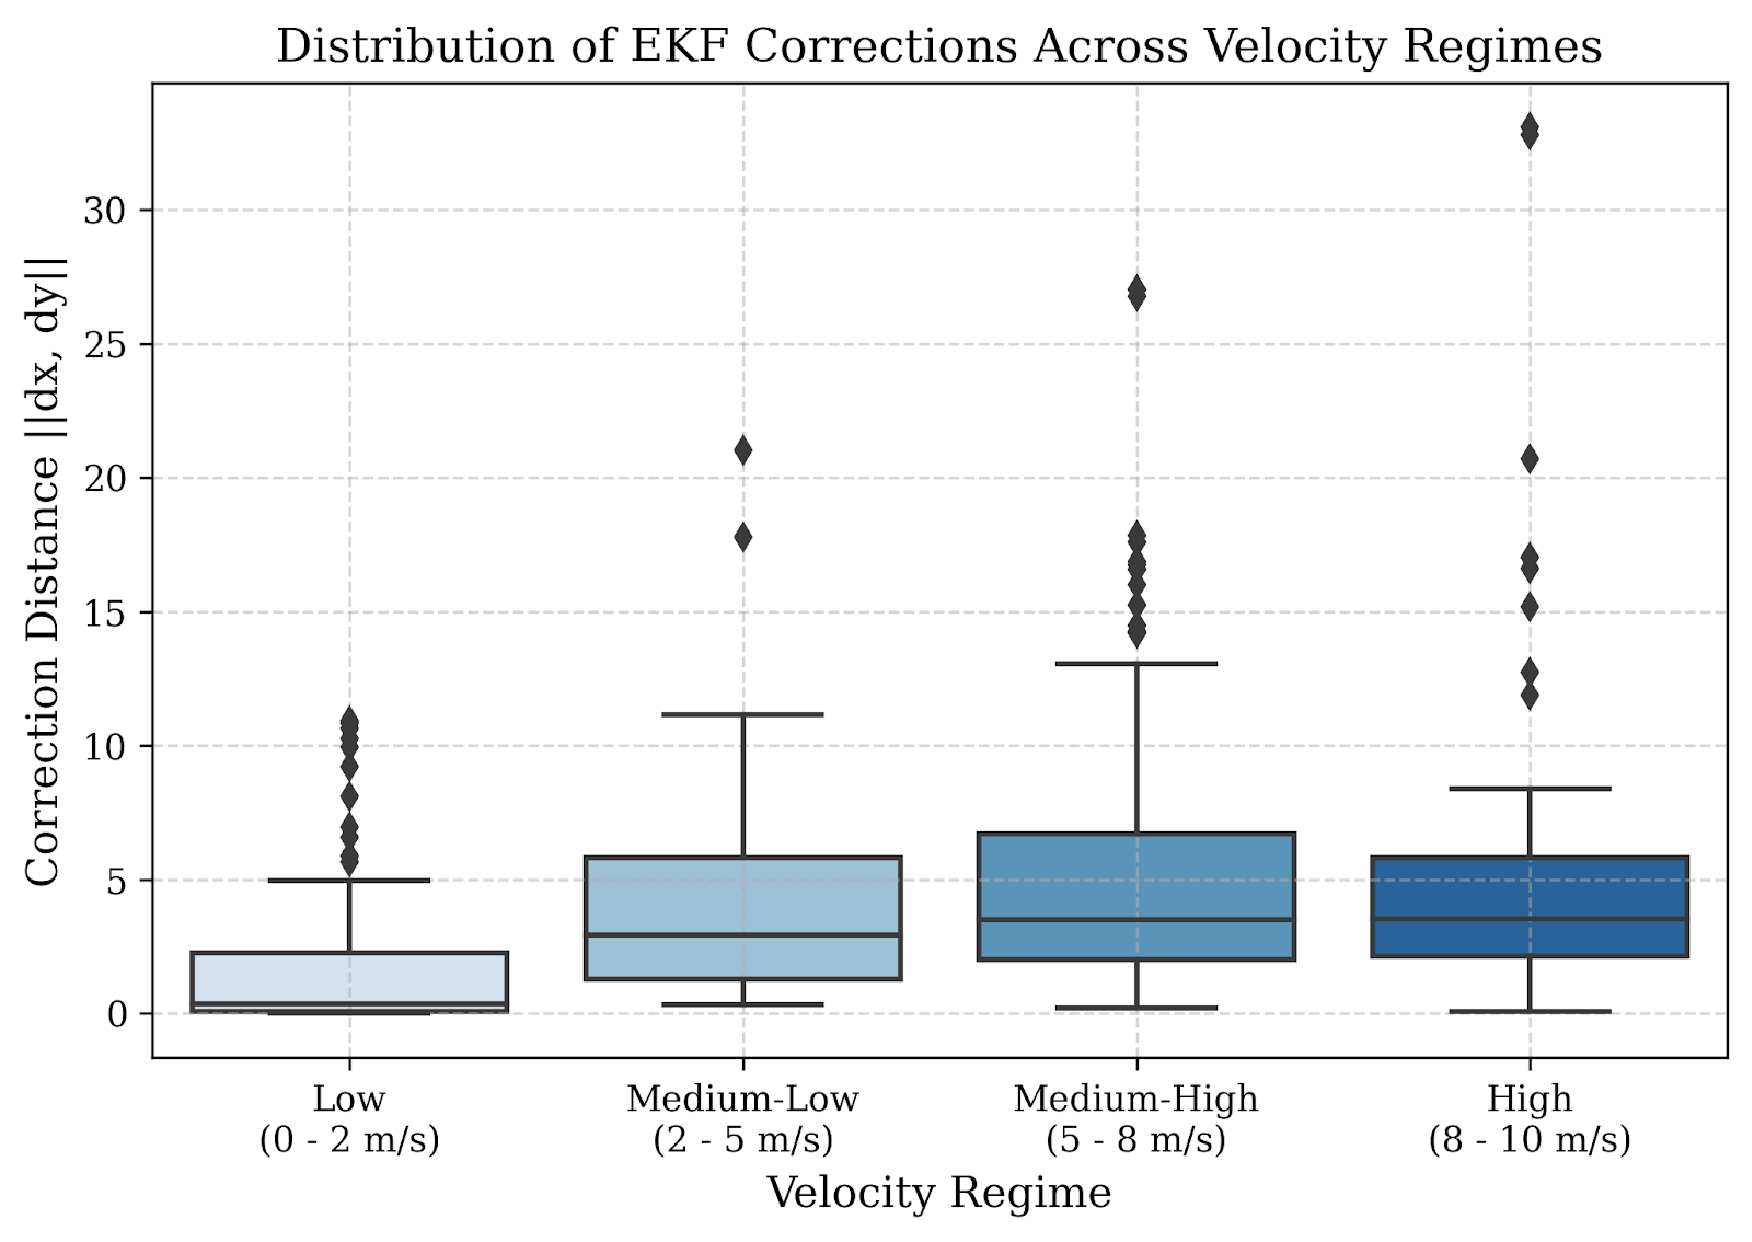
\includegraphics[width=0.8\textwidth]{figures/ekf_fig2_boxplot.pdf}
	\caption{\label{fig:ekf_boxplot}Distribution of EKF spatial corrections across four distinct velocity regimes, illustrating the upward shift in median and interquartile range at higher speeds.}
\end{figure}

This behavior is categorized across discrete speed brackets in Figure~\ref{fig:ekf_boxplot}. During high-velocity maneuvers ($>5.0\text{ m/s}$), the mean correction magnitude increases by over $180\%$ compared to idle regimes, with transient peak corrections reaching $33.10\text{ pixels/m}$.

% --- Figure 3: Temporal Alignment ---
\begin{figure}[t]
	\centering
	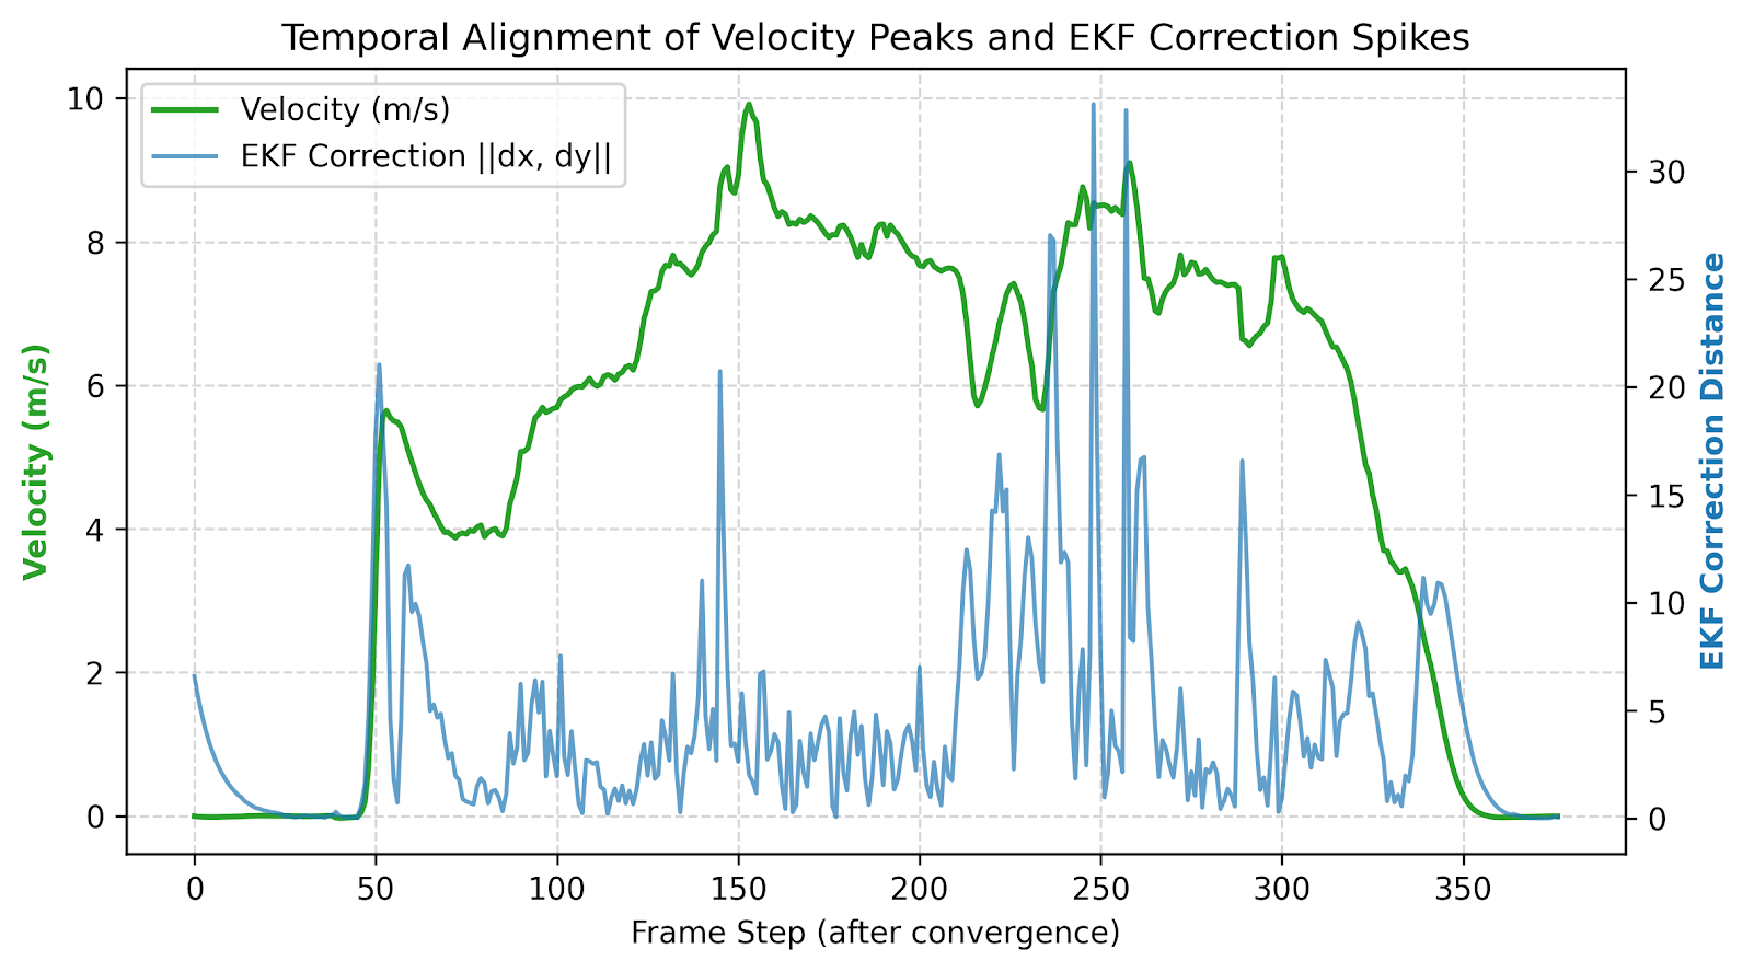
\includegraphics[width=0.85\textwidth]{figures/ekf_fig3_timeseries.pdf}
	\caption{\label{fig:ekf_timeseries}Temporal synchronization of vehicle velocity peaks (green) with EKF spatial correction intervention spikes (blue) over 377 post-convergence frames.}
\end{figure}

Rather than indicating filter instability, the temporal alignment displayed in Figure~\ref{fig:ekf_timeseries} provides quantitative proof of active kinematic damping. The continuous-time Constant Turn Rate and Velocity (\textsc{Ctrv}) dynamic model acts as a mathematical flywheel: while raw sensor observations experience severe spatial jitter during rapid acceleration, the filter dynamically intervenes precisely when velocity peaks occur.

% --- Figure 4: Spatial Trajectory Smoothing ---
\begin{figure}[t]
	\centering
	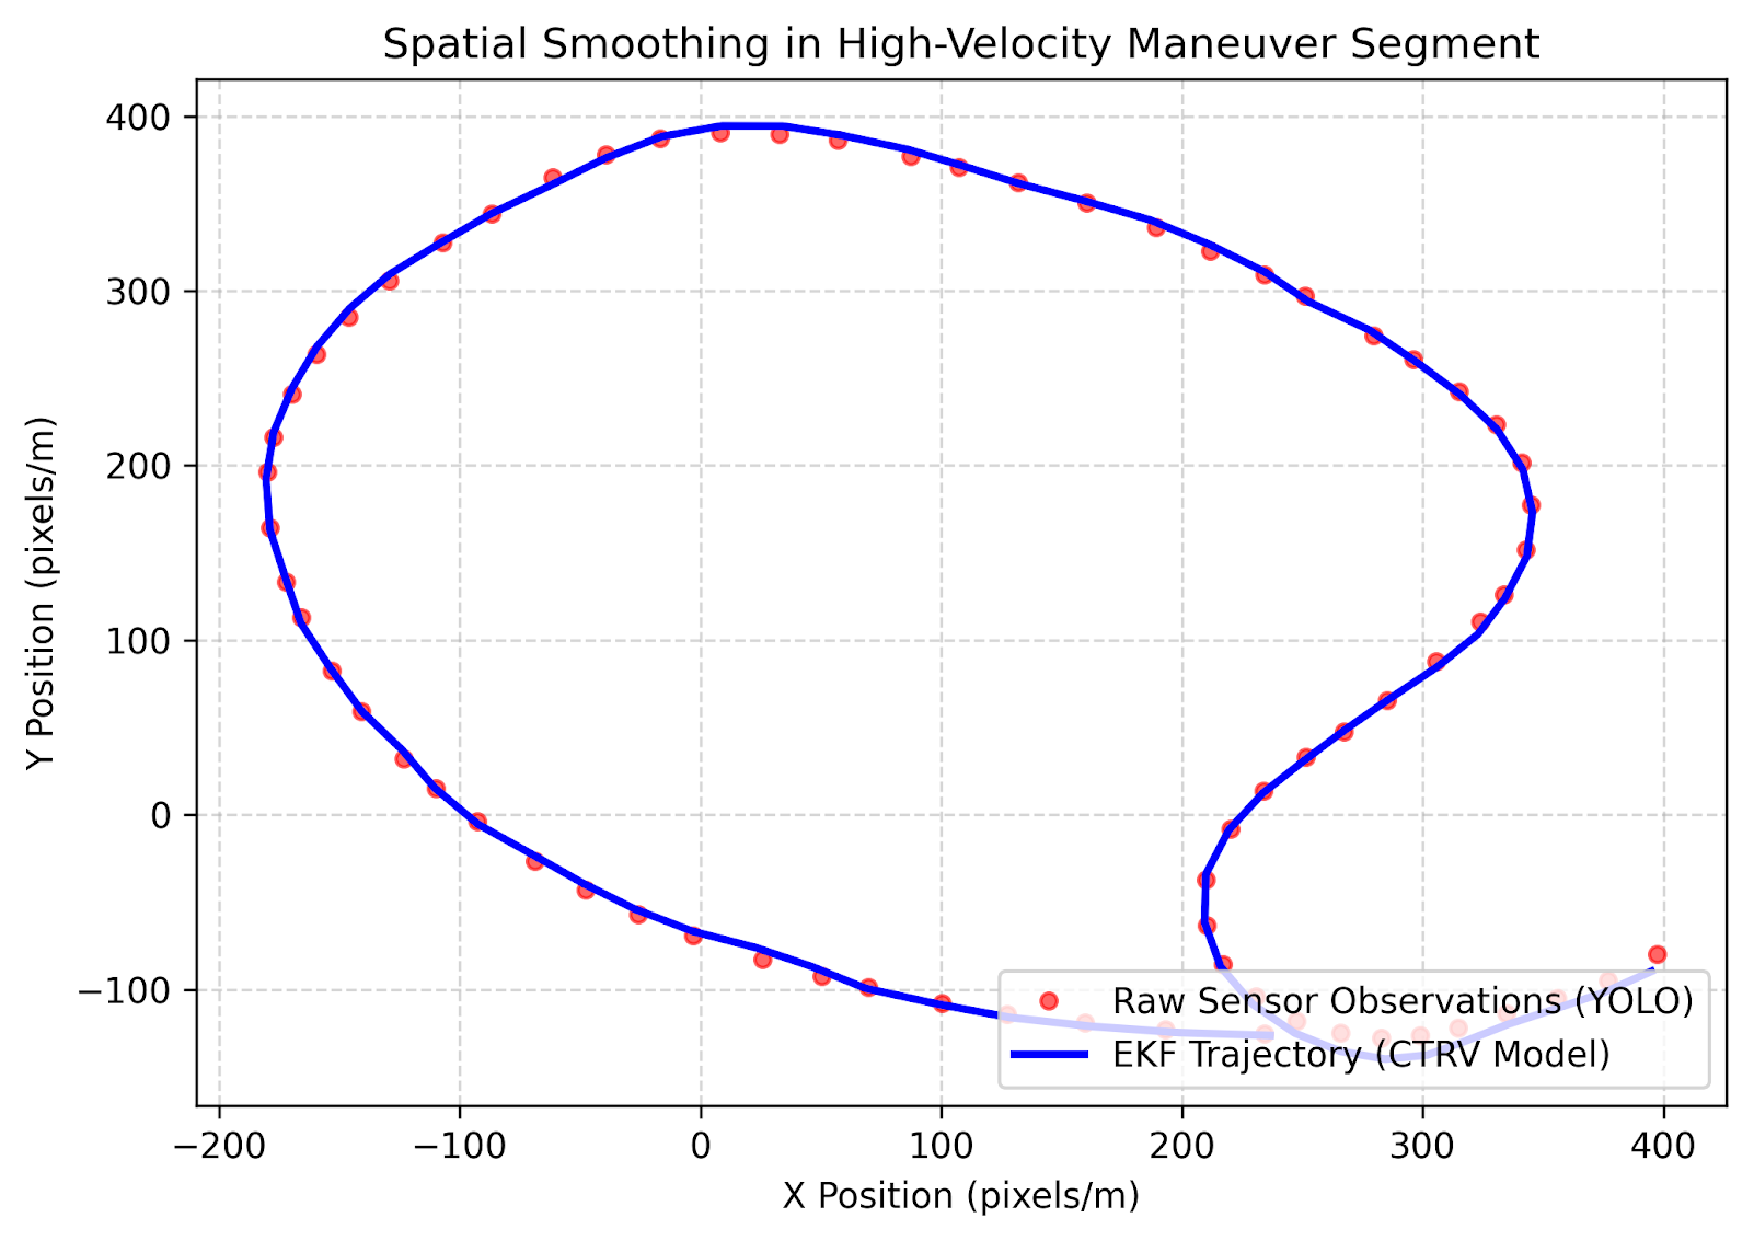
\includegraphics[width=0.8\textwidth]{figures/ekf_fig4_trajectory.pdf}
	\caption{\label{fig:ekf_trajectory}Spatial XY trajectory comparison during a high-speed maneuver segment (frames 150--220), highlighting the filter's ability to reject erratic raw sensor noise while maintaining physical momentum.}
\end{figure}

Finally, Figure~\ref{fig:ekf_trajectory} illustrates the spatial impact of this damping during a high-speed turning maneuver. The EKF propagates physical momentum forward, successfully isolating the true vehicular trajectory from high-frequency vision noise and bounding-box wobble.

\chapter{Code Optimizations and Functional Improvements}
\label{ch:code-optimization}

This chapter outlines the key optimizations applied to the bird's-eye-view vehicle detection framework, beyond the Extended Kalman Filter (EKF) integrations. These improvements focus on minimizing latency, refining mathematical models, and enhancing code maintainability.

\section{Code Execution and Performance Optimization}

\begin{itemize}
    \item \textbf{Video Stream Buffer Reduction}\\
    \textit{Impact:} Reduces the OpenCV \texttt{CAP\_PROP\_BUFFERSIZE} parameter from 2 to 1, minimizing frame queueing latency to ensure the YOLO model processes the absolute most recent frame.
    
    \textbf{Original Code:}
    \begin{lstlisting}[language=Python]
self.stream.set(cv2.CAP_PROP_BUFFERSIZE, 2)
    \end{lstlisting}
    
    \textbf{Improved Code:}
    \begin{lstlisting}[language=Python]
self.stream.set(cv2.CAP_PROP_BUFFERSIZE, 1)
    \end{lstlisting}

    \item \textbf{Movement Tracking and Responsiveness Diagnostics}\\
    \textit{Impact:} Introduces real-time processing lag calculation by comparing the current timestamp with the frame's origin timestamp. This diagnostic overlay (\texttt{lag\_ms}) allows for immediate visual feedback on end-to-end processing delay.
    
    \textbf{Original Code:}
    \begin{lstlisting}[language=Python]
# Not Present
    \end{lstlisting}
    
    \textbf{Improved Code:}
    \begin{lstlisting}[language=Python]
lag_ms = (time.time() - frame_time) * 1000
cv2.putText(annotated, f"Lag ={lag_ms:.4f} ms ", (30, 110),
            cv2.FONT_HERSHEY_SIMPLEX, 0.8, color, 2)
    \end{lstlisting}
\end{itemize}

\section{Pose Estimation and Math Improvements}

\begin{itemize}
    \item \textbf{Full 360\textdegree{} Orientation Calculation}\\
    \textit{Impact:} Removes the absolute value \texttt{abs()} wrappers around the axis projections. By preserving the mathematical signs (\(\pm\)) of the X and Y vectors, \texttt{np.arctan2} can compute the angle across all four quadrants (a full 360\textdegree{}). This eliminates the previous restriction where the vehicle's heading was limited to a 0--90\textdegree{} quadrant, drastically improving the true physical pose awareness.
    
    \textbf{Original Code:}
    \begin{lstlisting}[language=Python]
orientation_deg = np.degrees(np.arctan2(abs(proj_y), abs(proj_x)))
    \end{lstlisting}
    
    \textbf{Improved Code:}
    \begin{lstlisting}[language=Python]
orientation_rad = np.arctan2(proj_y, proj_x)
orientation_deg = np.degrees(orientation_rad)
    \end{lstlisting}

    \item \textbf{Fisheye Undistortion Balance Tuning}\\
    \textit{Impact:} Changes the fisheye balance parameter from 1.0 to 0.5. This provides a better compromise between retaining all original source pixels (Field of View) and eliminating the large black borders introduced during the mathematical rectification process.
    
    \textbf{Original Code:}
    \begin{lstlisting}[language=Python]
balance = 1
    \end{lstlisting}
    
    \textbf{Improved Code:}
    \begin{lstlisting}[language=Python]
balance = 0.5
    \end{lstlisting}

    \item \textbf{Kinematic Velocity Tracking}\\
    \textit{Impact:} Previously, the framework only extracted raw positional coordinates without any temporal motion history. By extracting the state vector from the newly integrated tracking module, the system now continuously computes and displays the vehicle's real-time velocity, unlocking advanced trajectory analysis.
    
    \textbf{Original Code:}
    \begin{lstlisting}[language=Python]
# Not Present (Only raw spatial position extracted)
    \end{lstlisting}
    
    \textbf{Improved Code:}
    \begin{lstlisting}[language=Python]
# Extract velocity from the EKF state vector (x[3])
velocity = ekf.x[3, 0]
cv2.putText(annotated, f"Vel={velocity:.2f} m/s", (30, 150),
            cv2.FONT_HERSHEY_SIMPLEX, 0.8, (255, 255, 0), 2)
    \end{lstlisting}
\end{itemize}

\chapter{Conclusion}
\label{ch:conclusion}

\textbf{Summary}\\
In this thesis, we built a real-time vehicle detection and tracking system using a single overhead fisheye camera to provide a bird's-eye view. By bringing together modern computer vision and deep learning, our system successfully tracks a vehicle's position, orientation, and speed on the fly. The complete pipeline handles everything from grabbing images and fixing fisheye distortion to using ArUco markers for mapping coordinates and YOLOv8 for recognizing the vehicles. To make the tracking even smoother and more reliable, we integrated an Extended Kalman Filter (EKF), which effectively cuts down on noise and keeps our state estimates consistent.

\textbf{Major Achievements \& Critical Assessment}\\
\label{sec:achievements}
Our experiments showed that the proposed approach works exceptionally well in practice. Here are the major achievements of our work:
\begin{itemize}
	\item \textbf{High Stability and Accuracy:} By fine-tuning the EKF during runtime and analyzing residuals, we achieved highly stable and accurate real-time tracking.
	\item \textbf{Reduced Jitter:} We significantly cut down on measurement jitter, ensuring smoother trajectory data.
	\item \textbf{Low Processing Latency:} The system runs efficiently enough to be viable for real-world miniature autonomous driving setups.
	\item \textbf{Robust Pipeline:} The overall architecture held up strong during our tests, combining motion thresholding and latency tracking to maintain performance.
\end{itemize}
While our setup does rely on visible ArUco markers and needs decent computing power to run YOLOv8, the results demonstrate that it is highly robust under the tested conditions.

\textbf{Related Topics}\\
This project touches on several exciting areas in the autonomous driving space, particularly visual odometry, tracking multiple objects at once, and running AI at the edge. The way we used YOLOv8 for real-time segmentation aligns with the latest trends in embedded vision, while our EKF implementation is a great practical example of classical state estimation and control theory in action.

\chapter{Future Scope of Work}
\label{ch:futurescope}

The work undertaken for the team project has been in continuation of a Master thesis work completed by a previous students. The architectural design of the foundational steps had provided certain boundary conditions for the overlaying work of pose estimation. The future scope includes incremental changes in both areas of this work.

\begin{enumerate}[label=\textbf{Area \arabic*:}, leftmargin=*, itemsep=1em] 
	\item \textbf{Inference Latency :} The primary reason for latency in the system has been accredited to the high parameter count of the YOLO model used for the object detection pipeline. The million parameter model can be substituted by a lightweight task focused strategically trained model. The computational efficiency of the camera architecture and the inference speed should be considered while making this selection. The model training can be elevated by larger size of annotated datasets created using foundational annotating models like SAM,DINO etc.
	
	\item \textbf{ArUCo Markers :} The dependency of the localization pipeline on external landmarks such as the ArUCo markers can be eliminated with the use of detection of map characteristics including but not limited to the lanes, corners or external peripheral dimensions of the grey map. The flexibility provided by this should improve generalization of the localization algorithm.
	
	\item \textbf{Hardware Restrictions :} The secondary reason for lower inference speeds is the large size of the processing frames passed to the model. This size is a consequence of the ratio of object size to the camera's field of vision. The lower occupancy of pixels is an obstacle which could be overcome by restricting field of vision to dedicated zones or using a faster processing device to generate the high quality frames.
	
	\item \textbf{Software Architecture :} The code has been implemented in a python environment with no influential use-case of objected oriented programming approach. This could be substituted by changing to Tensorflow and Keras based model training with ONNX wrapper and inference in C++ environment, which is a memory efficient and better suited area for real-time operating systems.
	

\end{enumerate}
%\input{chapters/chapter3.tex}
%\input{chapters/chapter4.tex}
%\input{chapters/chapter5.tex}


%----------------------------------------------------------------------------------------
%	THESIS CONTENT - APPENDICES
%----------------------------------------------------------------------------------------

% By using input instead of include for the chapters we are able to move the following line here
% Therefore the addition before the last chapter is not necessary anymore.

% Call the following chapters "Appendix" inside the table of contents
\addtocontents{toc}{\string\def\string\chaptername{Appendix}}

\appendix % Cue to tell LaTeX that the following "chapters" are Appendices

% Ensure proper section numbering in appendix, e.g., A.1, A.2, B.1, …
\renewcommand{\thesection}{\thechapter.\arabic{section}}
\renewcommand{\thesubsection}{\thesection.\arabic{subsection}}
\renewcommand{\thesubsubsection}{\thesubsection.\arabic{subsubsection}}

%%% CHANGES NEEDED HERE
%
% Include the appendices of the thesis as separate files from the Appendices folder
% Uncomment the lines as you write the Appendices

%% Appendix A
 
\chapter{References}
\label{appendixa}

\section{References}

\begin{itemize}
\item Colloquial style: “Computation power has skyrocketed in the last few years.”
\item Widespread knowledge: “The Internet is becoming more and more important.”
\item Superlatives: “One of the most beautiful concepts,” “great possibilities.”
\item Be careful with strong claims: “the only possibility,” “the best solution,” “impossible.”
\end{itemize}
%\include{appendices/appendixB}
%\include{appendices/appendixC}



%----------------------------------------------------------------------------------------
%	BIBLIOGRAPHY
%----------------------------------------------------------------------------------------

% Bibliography has no wide margins:
\newgeometry{
	inner=2cm, % Inner margin
	outer=2cm, % Outer margin
	marginparwidth=0cm,
	marginparsep=0mm,
	bindingoffset=.5cm, % Binding offset
	top=1.5cm, % Top margin
	bottom=2.5cm, % Bottom margin,
	includehead,
	includefoot
	% showframe, % Uncomment to show how the type block is set on the page
}

\addchap{References}

% enables two-column layout for bibliography
\setlength\columnsep{2em}
\begin{multicols}{2}
	\begin{refcontext}[sorting=nyt] % sort bibliography by last name, year, title
		\renewcommand*{\bibfont}{\small\RaggedRight}
		\linespread{1.0}\selectfont % increase linespread if desired (not recommended)
		\printbibliography[heading=none]
	\end{refcontext}
\end{multicols}

%----------------------------------------------------------------------------------------

\end{document}
